\documentclass[12pt,letterpaper]{article}
\usepackage[left=1in,top=1in,right=1in,bottom=1in,nohead]{geometry}
\pagestyle{empty}
\linespread{1.5}
\usepackage[T1]{fontenc}
\usepackage{ragged2e}
\usepackage{setspace}
\usepackage{mdwlist}
% \usepackage{array}
% \usepackage{multirow}
\usepackage{graphicx}
% \usepackage{wrapfig}
% \usepackage{longtable}
% \usepackage{subfig}
\usepackage{amsmath}
\usepackage{amssymb}
\usepackage{bbm}
\usepackage{dsfont}
\usepackage{mathptmx}
\usepackage[hang]{caption}
\DeclareMathAlphabet{\mathcal}{OMS}{cmsy}{m}{n}
\usepackage{relsize}
\usepackage{fancyvrb}
\def \fullline {\vspace{.2em}\hrule\vspace{3px}}

\begin{document}
\tableofcontents
\setlength{\parindent}{0.25in}
\setlength{\floatsep}{0in}
\section{Radial Density Function}
\subsection{Calculation of Distances with Periodicity}
Suppose a large chemical structure has uncountably many atoms but the follow a
periodic pattern of $n$ atoms every $p$ Angstroms. The atom locations within a
period are given by $a_1, a_2, \ldots, a_n$ where $a_i \in \mathbb{R}^3$. The
radial density function is the distribution of pairwise distances between these
atoms.

The distances $d$ between atoms $a_i$ and $a_j$ where $i \neq j$, atom $a_i$
has been displaced by $x$, and atom $a_j$ has been displaced by $y$ per the
periodicity is 
\begin{align*}
  d^2 &= \langle a_i + x - (a_j + y), a_i + x - (a_j + y) \rangle \\
      &= \langle a_i-a_j, a_i-a_j \rangle  + \langle x-y, x-y \rangle  
      + 2 \langle a_i-a_j,x-y \rangle 
\end{align*}
where $x =(k_1 p, k_2 p, k_3 p)$ for $k_i \in \mathbb{Z}$ 
and $y = (l_1 p, l_2 p, l_3 p)$ for $l_i \in \mathbb{Z}$.
Here $\langle x,y \rangle $ denotes the inner product between $x$ and $y$. 

Suppose $D$ is a random variable that samples at random the distances, $d$, in
the chemical structure. The radial density function is the probability density
function of this random variable. This function can be estimated empirically via
a histogram.

The histogram is then normalized by the volume a spherical shell.
\begin{align*}
  \frac{4}{3} &\pi (r + \Delta r)^3 - \frac{4}{3} \pi r^3\\
     &=\frac{4}{3} (3 r^2 \Delta r + 3 r (\Delta r)^2 + (\Delta r)^3) \\
              &\approx 4 \pi r^2 \Delta r
\end{align*}
where $\Delta r$ tends to zero.

For a histogram with frequency, $f$, for bin $[d_i, d_{i+1}]$, we replace $f$
with $f / d_i^2$. And then normalize the histogram so that the sum over all bins
is one.

\subsection{Adding Noise For Atom Vibration}
Due to the vibrations of the molecules, the radial density function will not be
just the equilibrium positions. We can approximate this fluctuation in distances
via a Gaussian filter or Weierstrass transform.

\begin{align*}
F(x)=\frac{1}{\sqrt{4\pi t}} 
  \int_{-\infty}^\infty f(y) e^{-\frac{(x-y)^2}{4t}} dy
\end{align*}

Given that the density function is only defined for a finite number of
distances, we use a discrete version of the transform making sure to keep the
sum of the weights equal to one.

\begin{align*}
  F(d_k) = \frac{\sum_{d_i = d_0}^{d_n} f(d_i) \exp\left(-\frac{(d_k -
                  d_i)^2}{4t}\right)}
            {\sum_{d_i = d_0}^{d_n} \exp\left(-\frac{(d_k - d_i)^2}{4t}\right)}
\end{align*}
where $d_0$ is the minimum distance and $d_n$ is the maximum distance.

\subsection{Cubane Example}
As an example of the above, below are the calculations for cubane ($C_8 H_8$).\\

\noindent Here are the coordinates of the elements in cubane in Angstroms.

\begin{verbatim}
Element, x, y, z
C, 1.2455, 0.5367,-0.0729
C, 0.9239,-0.9952, 0.0237
C,-0.1226,-0.7041, 1.1548
C, 0.1989, 0.8277, 1.0582
C, 0.1226, 0.7042,-1.1548
C,-0.9239, 0.9952,-0.0237
C,-1.2454,-0.5367, 0.0729
C,-0.1989,-0.8277,-1.0582
H, 2.2431, 0.9666,-0.1313
H, 1.6638,-1.7924, 0.0426
H,-0.2209,-1.2683, 2.0797
H, 0.3583, 1.4907, 1.9059
H, 0.2208, 1.2681,-2.0799
H,-1.6640, 1.7922,-0.0427
H,-2.2430,-0.9665, 0.1313
H,-0.3583,-1.4906,-1.9058
\end{verbatim}

\subsubsection{Cubane Radial Density Functions}
\begin{figure}[ht!]
  \begin{center}
    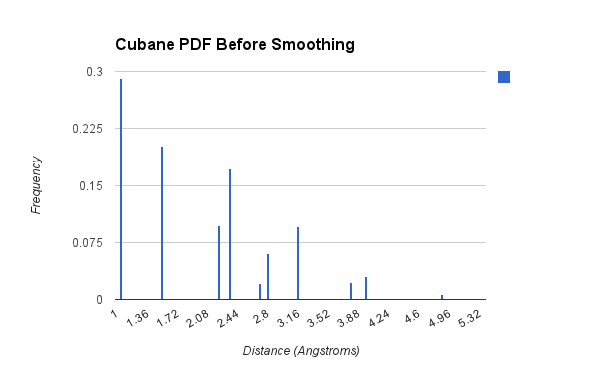
\includegraphics[scale=0.7]{figs/cubane_rdf_before_smoothing.png}
    \caption{Before Smoothing}
  \end{center}
\end{figure}

\begin{figure}[ht!]
  \begin{center}
    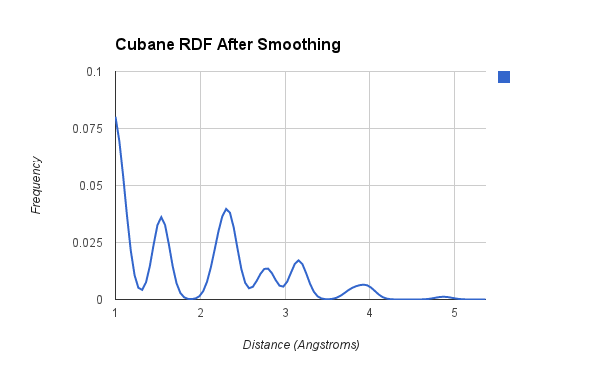
\includegraphics[scale=0.7]{figs/cubane_rdf_after_smoothing.png}
    \caption{After Smoothing}
  \end{center}
\end{figure}
\clearpage

\subsection{Experimental and Theoretical RDFs for Known Structures}
For some structures, we are able to theoretically calculate the RDF from atom
locations and also have the experimental RDF from Xray scattering. These known
matches provide some insight into understanding how the experiments and theory
align. The RDF comparison are shown below.

Outside of these structures, there are not many other known matches. There are a
few reasons for this. First, if a structures is already known at the atomic
level then there is no need to run an xray diffraction experiment. Second, if a
structure is periodic as in a lattice, the atomic structure can be determined by
xray diffraction which is easier and cheaper than xray scattering.

\subsubsection{Ga As}
\noindent Experimental Data: Pair Distribution Functions Analysis, Valeri
Petkov\\
\noindent Calculated Data: Maria Chan\\
\begin{figure}[ht]
  \begin{center}
    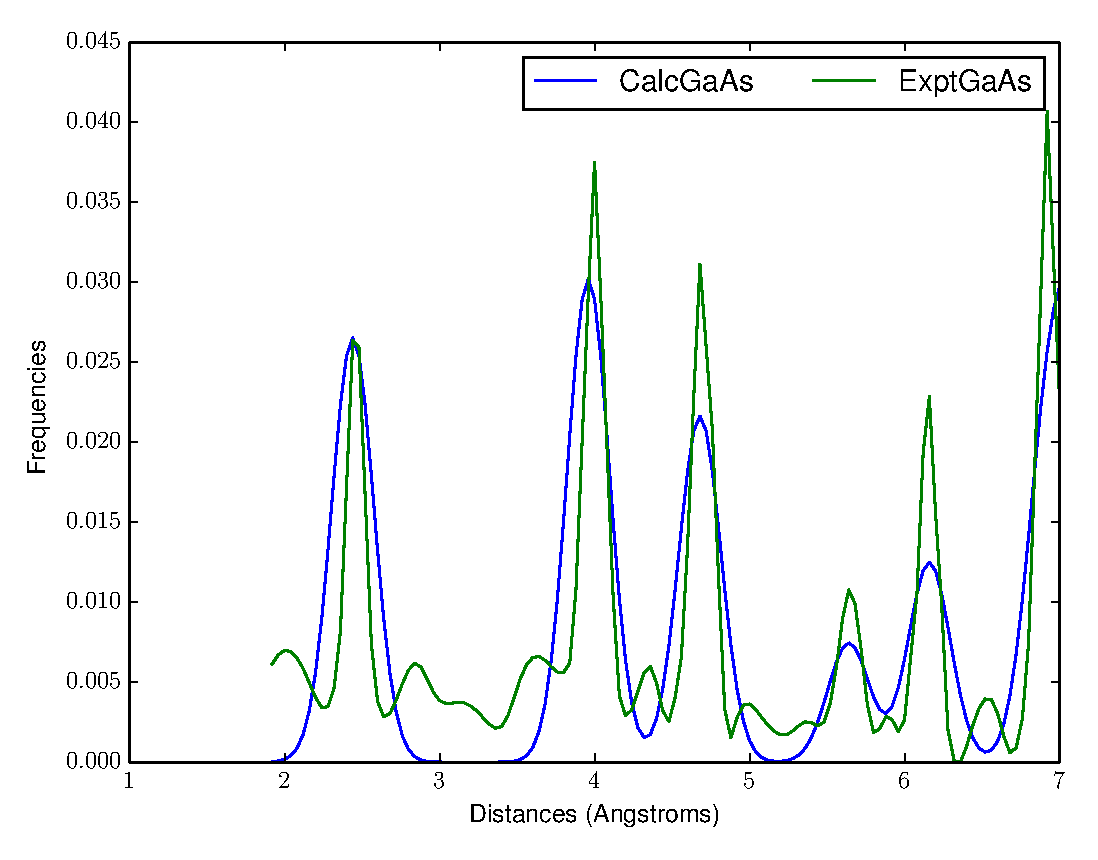
\includegraphics[scale=0.7]{figs/gaas_pdf_comparison.eps}
    \caption{Ga As}
  \end{center}
\end{figure}

\subsubsection{In As}
\noindent Experimental Data: Pair Distribution Functions Analysis, Valeri
Petkov\\
\noindent Calculated Data: Maria Chan\\
\begin{figure}[ht]
  \begin{center}
    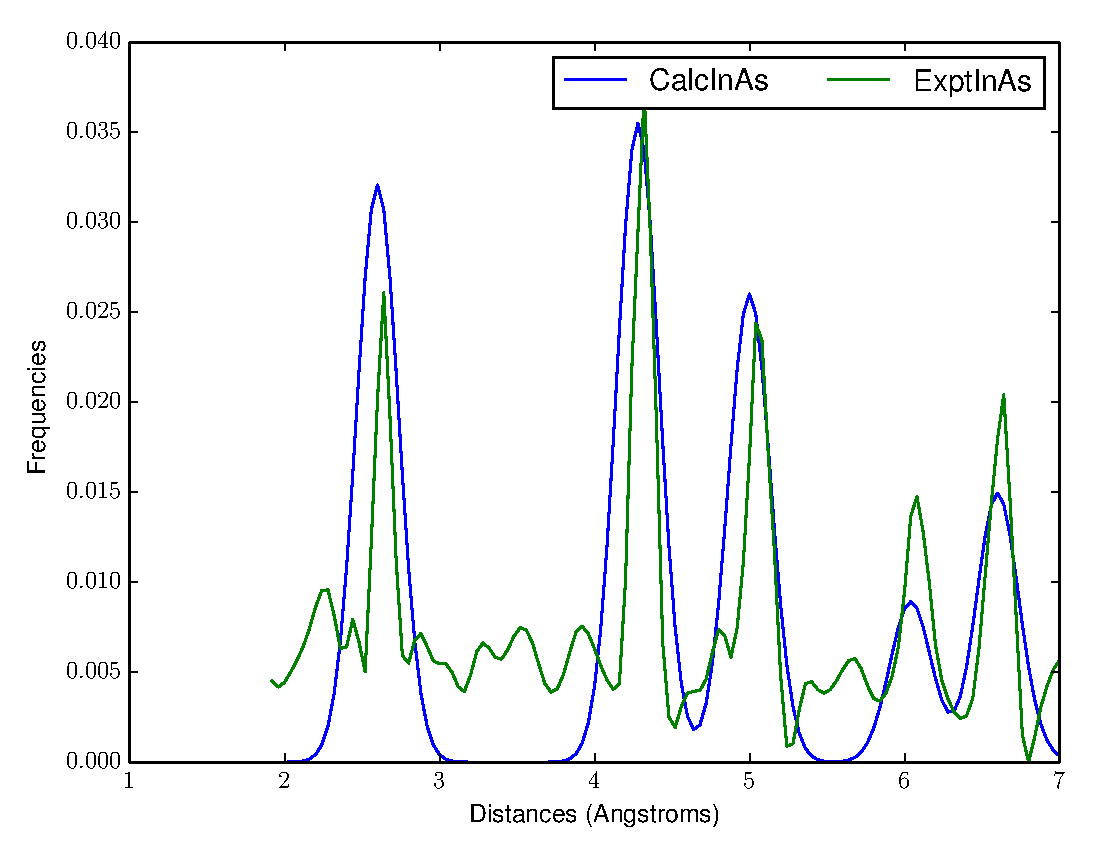
\includegraphics[scale=0.7]{figs/inas_pdf_comparison.eps}
    \caption{In As}
  \end{center}
\end{figure}

\subsubsection{Si Lattice}
\noindent Experimental Data: J. AM. CHEM. SOC. VOL. 133, NO. 3, 2011, P:
503-512\\
\noindent Calculated Data: http://materialsproject.org/materials/mp-149/ \\
\begin{figure}[ht]
  \begin{center}
    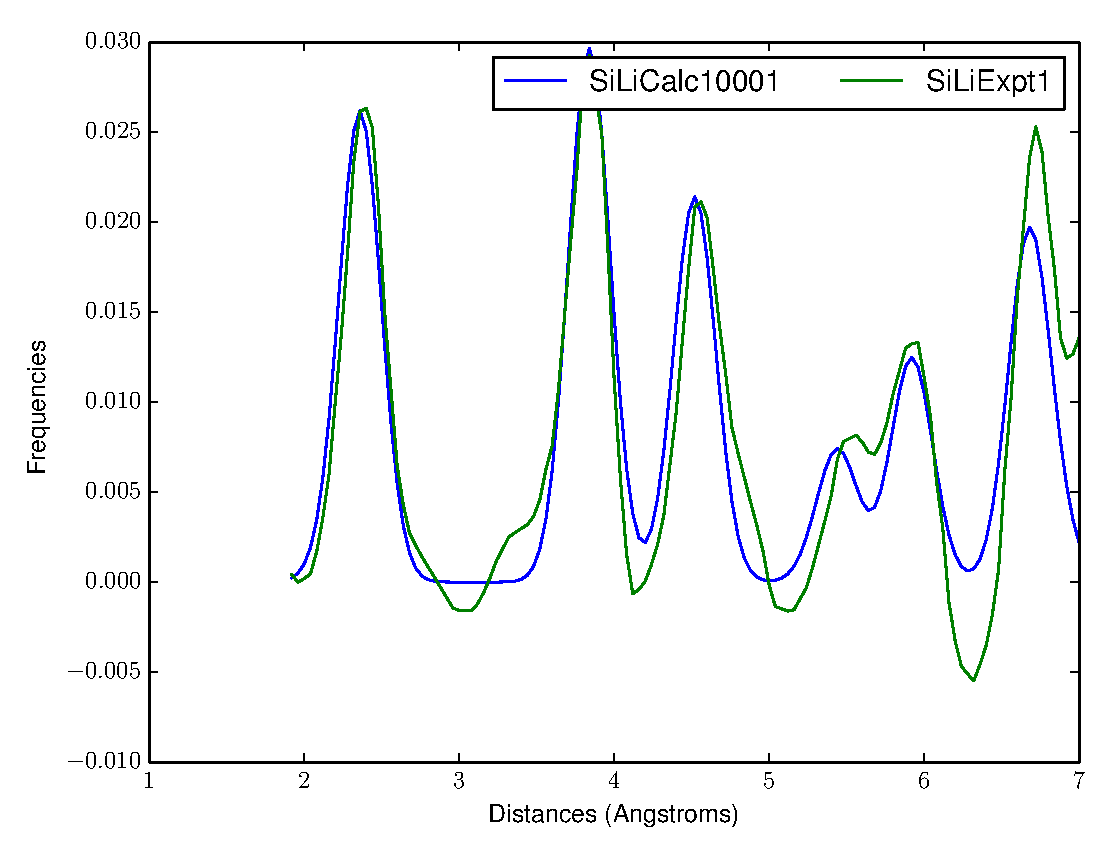
\includegraphics[scale=0.7]{figs/SmoothCalibrationSiLiCalc10001-SiLiExpt1.eps}
    \caption{Si Lattice}
  \end{center}
\end{figure}
\pagebreak

\section{Smoothing Analysis}
Consider a function, $SmoothAndNormalize(i, t)$, that smoothes the image, $i$,
with a smoothing coefficient of $t$ and then normalizes the smoothed image so
that the weights sum to one. To calibrate the smoothing coefficient, we focus on
the SiLi calculated and experimental matches, SiLiCalc10001 and SiLiExpt1. We
want to find the smoothing coefficient, $t$, that after smoothing and
normalization the calculated image is the closest match to the experimental
image.
\begin{align*}
  \hat{t} = \underset{t}{\arg\min} \| X -
    SmoothAndNormalize(C, t) \|_2
\end{align*}

where $\|\cdot\|_2$ is the $L^2$ norm, $X$ is the experimental image, and $C$ is
the calculated image.

We found that $\hat{t} = 0.0092$.

\begin{figure}[ht]
  \begin{center}
    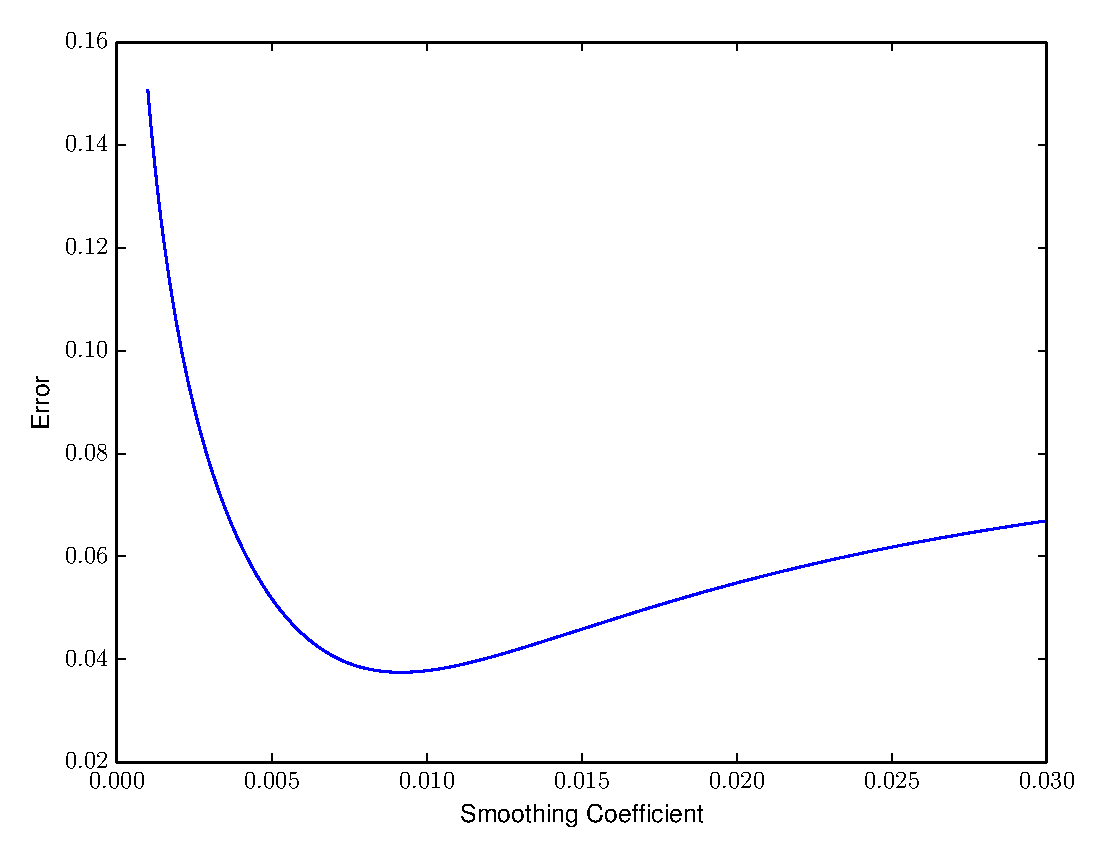
\includegraphics[scale=0.8]{figs/SmoothingCalibrationCurve.eps}
    \caption{Smoothed - Expt Error vs Smoothing Coefficients}
  \end{center}
\end{figure}

\begin{figure}[ht]
  \begin{center}
    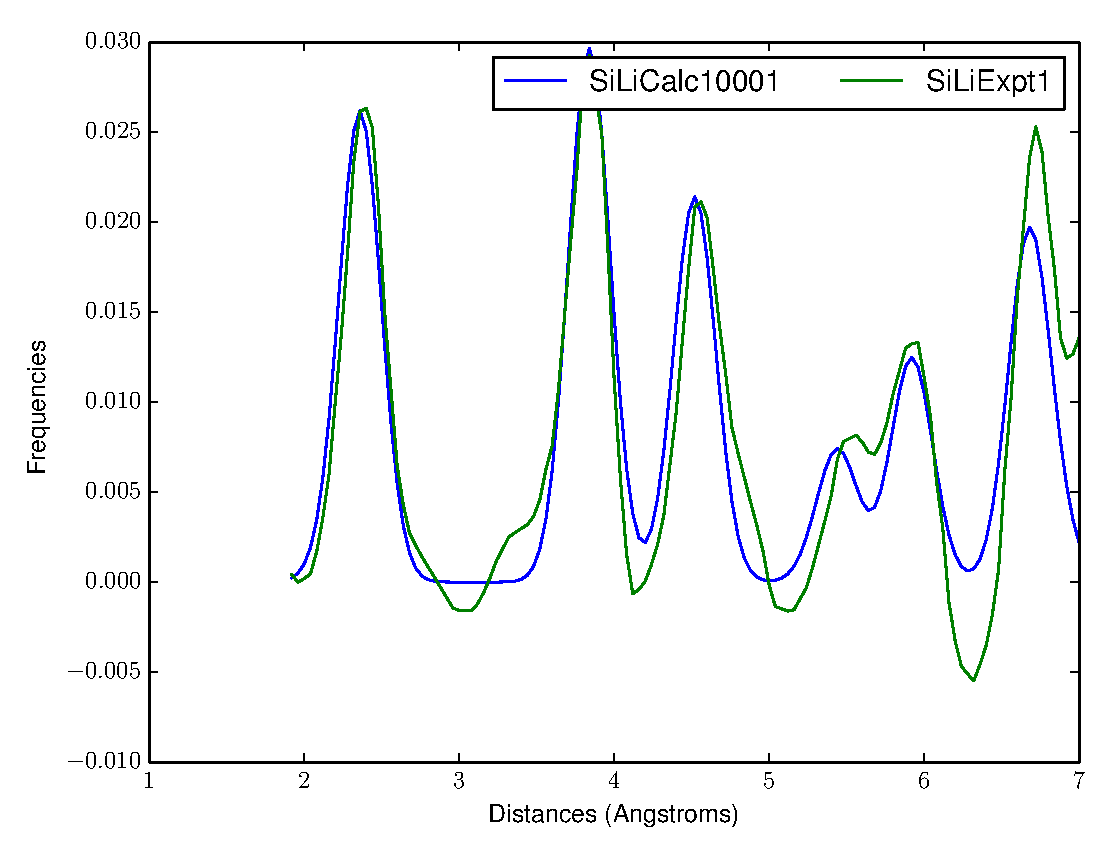
\includegraphics[scale=0.8]{figs/SmoothCalibrationSiLiCalc10001-SiLiExpt1.eps}
    \caption{Smoothed SiLiCalc10001 vs SiLiExpt1}
  \end{center}
\end{figure}

\clearpage

\section{Matching Algorithm Evaluation \label{s:algo_eval}}

The goal of this project is to invent an algorithm that will find the best
matching calculated image for a given experimental image. A more audacious goal
is to find an algorithm that can decompose experimental image into a linear
combination of a few calculated image.

Before running an experiment, it is possible to theoretically predict the
feasible structures that could occur during the experiment. Given this matching
algorithm, during the experiment, we could match the experimental results back
to the theoretically predicted structures. This would give an 'x-ray vision' into
the structures, being able to see that atom locations as the experiment
progresses.

One way to evaluate the performance of a proposed matching algorithm is to use
the set of known experimental and calculated matches. Taking the set of
calculated images as a whole, the algorithm should be able to recover the
calculated match given the experimental image. 

The problem with this evaluation metric is that there are only three known
calculated/experimental matches. This is not a large enough number of samples
for good statistics. The reason there are not too many matching pairs is because
the known structures at this time are periodic and can be observed
experimentally through cheaper x-ray diffraction experiments. Non-periodic
structures which are the focus of this project are studied precisely because
their exact structures are not known.

An alternative approach to using the calculated and experimental matching pairs
directly is to simulate experimental images by adding random noise to a
calculated image. The goal then becomes to recover the original calculated image
given the simulated experimental image.

\begin{figure}[ht]
  \begin{center}
    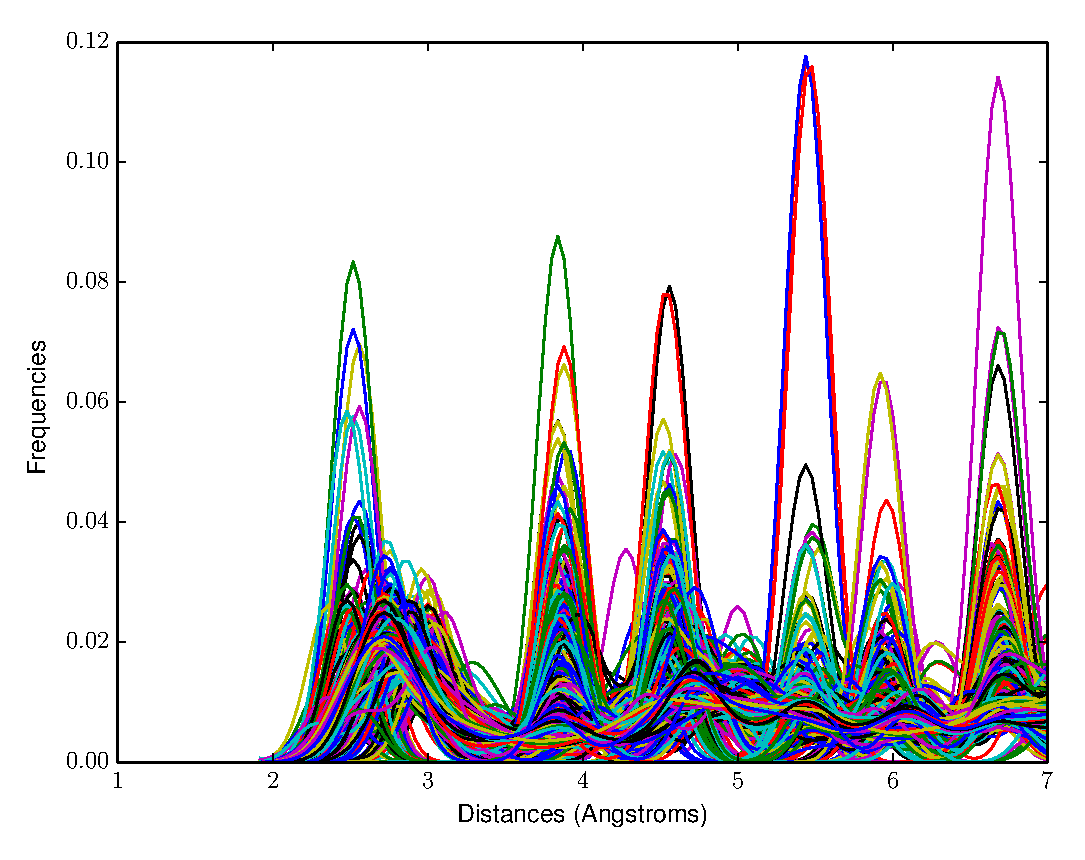
\includegraphics[scale=0.7]{figs/AllCalcImages.eps}
    \caption{All Calculated Images}
  \end{center}
\end{figure}

\begin{figure}[ht]
  \begin{center}
    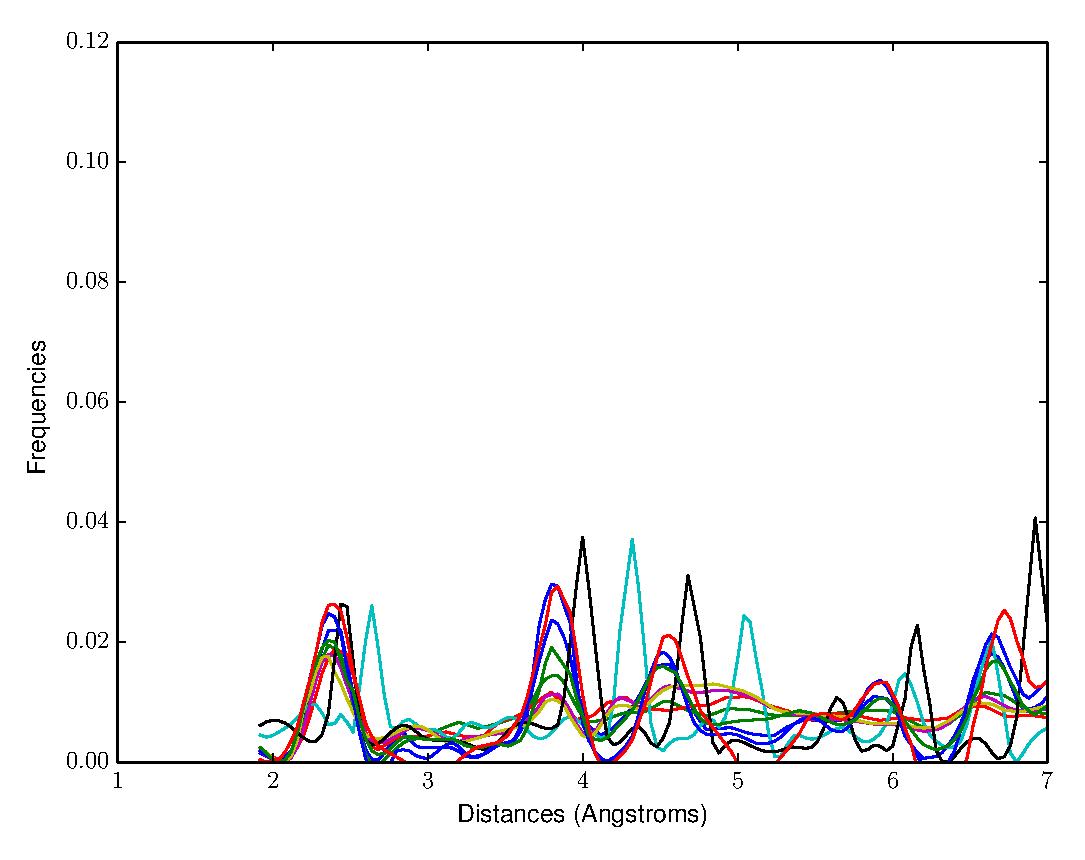
\includegraphics[scale=0.7]{figs/AllExptImages.eps}
    \caption{All Experimental Images}
  \end{center}
\end{figure}

\clearpage

\subsection{Noise Analysis}
The experimental images present three different varieties of noise compared to
the calculated images.

\begin{itemize}
  \item{Tilt: Consider the baseline of the image to be the piecewise line
      connecting the valleys of the image. The experimental images seem to have a
      non-zero and slanted baseline compared to the calculated images which 
      have a baseline at zero.} 
  \item{Noise: Between the major peaks of the experimental images, there are
      also several minor peaks. These minor peaks are not found in the calculated
      images.}
  \item{Peak Heights Difference: The heights of the major peaks vary between the
      calculated and experimental images.}
\end{itemize}

\begin{figure}[ht]
  \begin{center}
    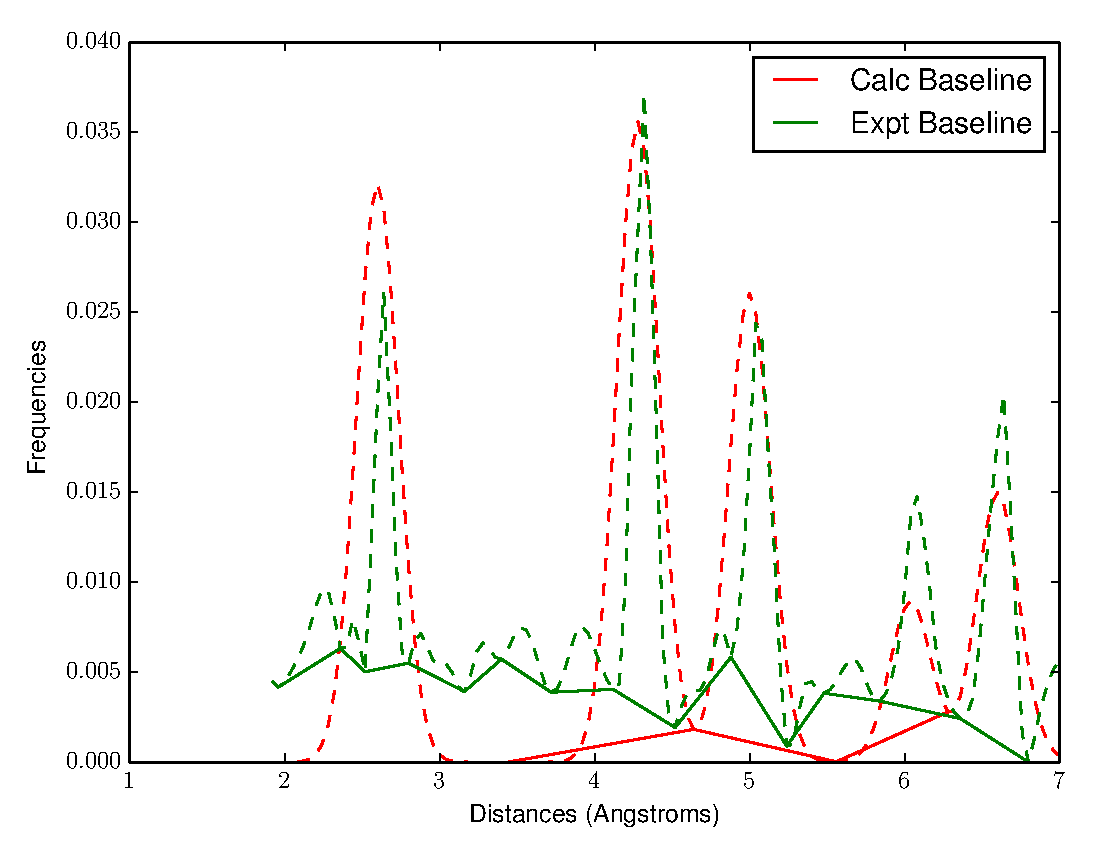
\includegraphics[scale=0.7]{figs/inas_valleys.eps}
    \caption{In As}
  \end{center}
\end{figure}

To simulate these features, I first estimated the distributions of the number of
peaks, peak locations, and the noise peak heights. 

\subsubsection{Peak Counts}
To estimate the distribution of number of peaks per image, I took all of the
experimental images and estimated the number of peaks. Then I visually inspected
the histogram to estimate the distribution.

From the histogram, I concluded that the number of peaks is uniformly
distributed between 7 and 15.

\begin{figure}[ht]
  \begin{center}
    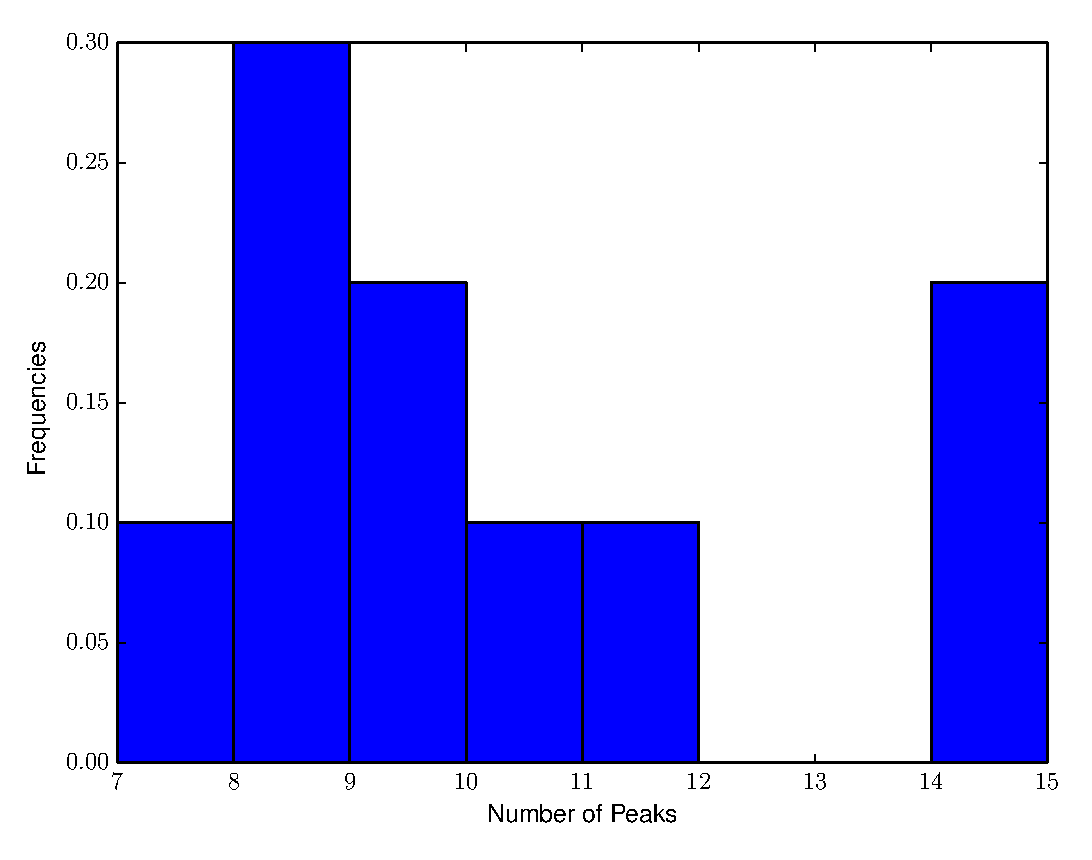
\includegraphics[scale=0.8]{figs/peak_counts_hist.eps}
    \caption{Peak Count Distribution}
  \end{center}
\end{figure}

Note that the estimation is strongly dependent on the maximum length of the
image. The raw InAs spectrum goes out to 10 angstroms and has much more than 15
peaks.

\begin{figure}[ht]
  \begin{center}
    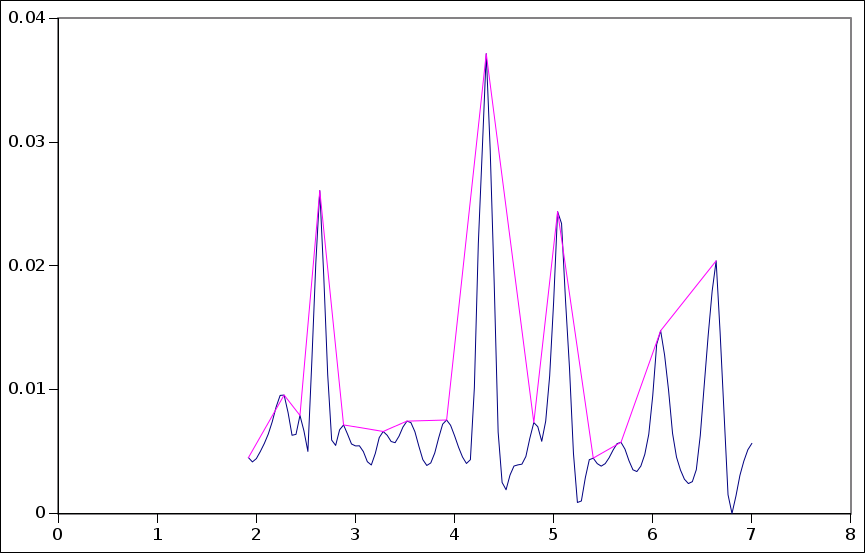
\includegraphics[scale=0.5]{figs/inas_peaks_7ang.png}
    \caption{InAs Expt, Max 7 Angstroms}
  \end{center}
\end{figure}

\begin{figure}[ht]
  \begin{center}
    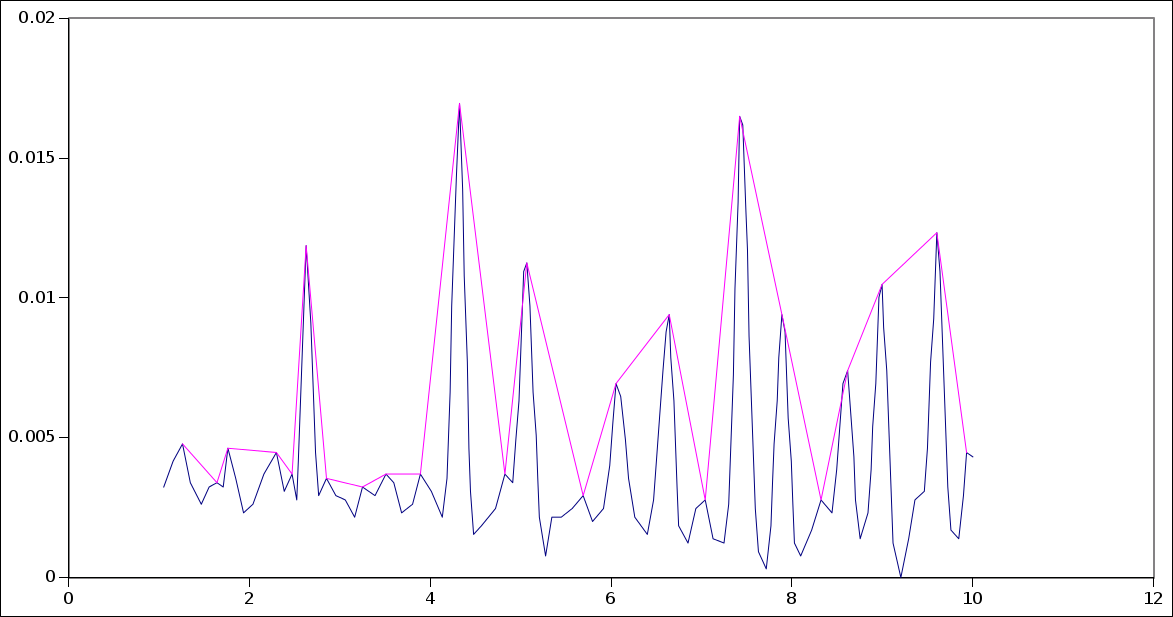
\includegraphics[scale=0.4]{figs/inas_peaks_10ang.png}
    \caption{InAs Expt, Max 10 Angstroms}
  \end{center}
\end{figure}
\clearpage

\subsubsection{Peak Locations}
To estimate the distribution of the location of the peaks, I first took all of
the experimental images and calculated the distances of all of the peaks. Then I
charted this as a histogram to visually inspect the distribution.

From the histogram, I concluded that the locations are uniformly distributed
between 1.96 and 7.
\begin{figure}[ht]
  \begin{center}
    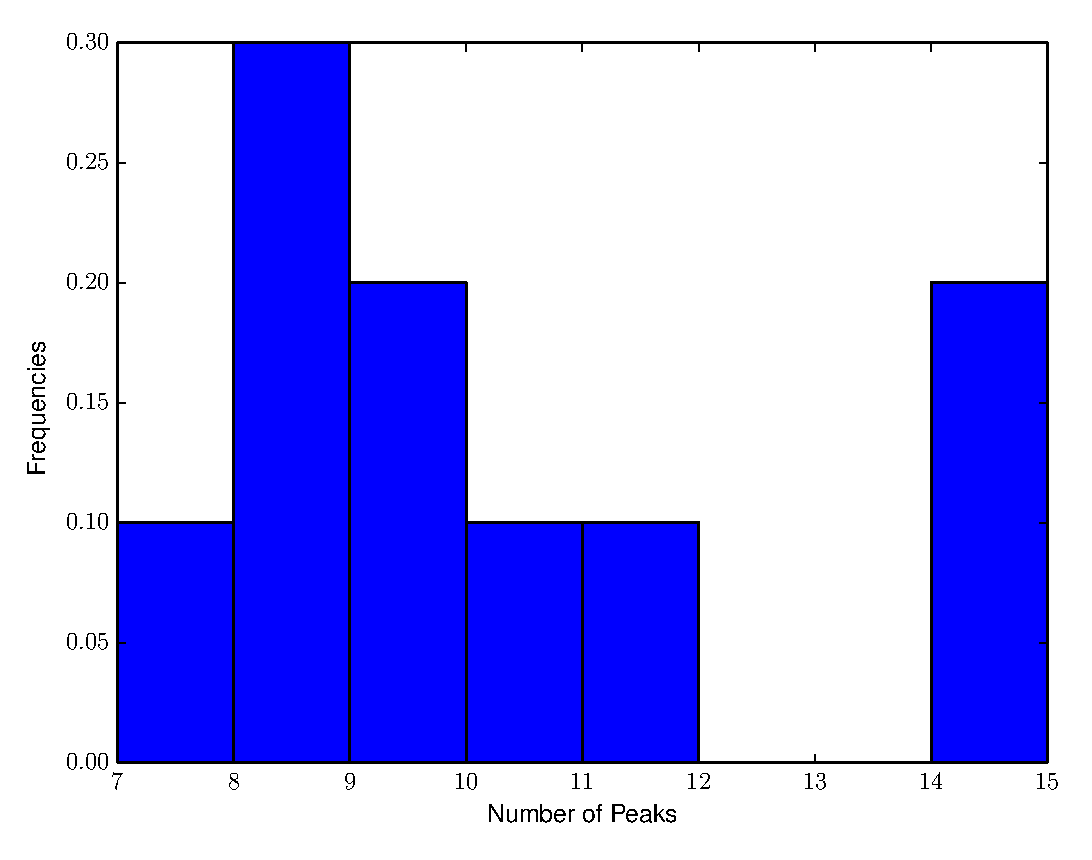
\includegraphics[scale=0.8]{figs/peak_counts_hist.eps}
    \caption{Peak Location Histogram}
  \end{center}
\end{figure}
\clearpage

\subsubsection{Noise Peak Heights}
To add noise to the image, I random noise directly to the original frequencies.
That is, $N = I + R$, where $N$ is a vector of frequencies for the noisfied
image, $I$ is for the original image, and $R$ is for the random noise.

In light of this, to estimate how much noise to add, I first calculated $E = X -
C$, where $E$ is the error or noise to be added, $X$ is the experimental image,
and $C$ is the calculated image. I considered the errors at different distances
to be independent and thus considered all of the errors to be for any distance.
Taking all of the errors together, I estimate the error distribution. From the
histogram and cumulative distribution function, I concluded that the error
distribution is most similar to a normal distribution. The estimate for the mean
is 0.004 and standard deviation is 0.004.

\begin{figure}[ht]
  \begin{center}
    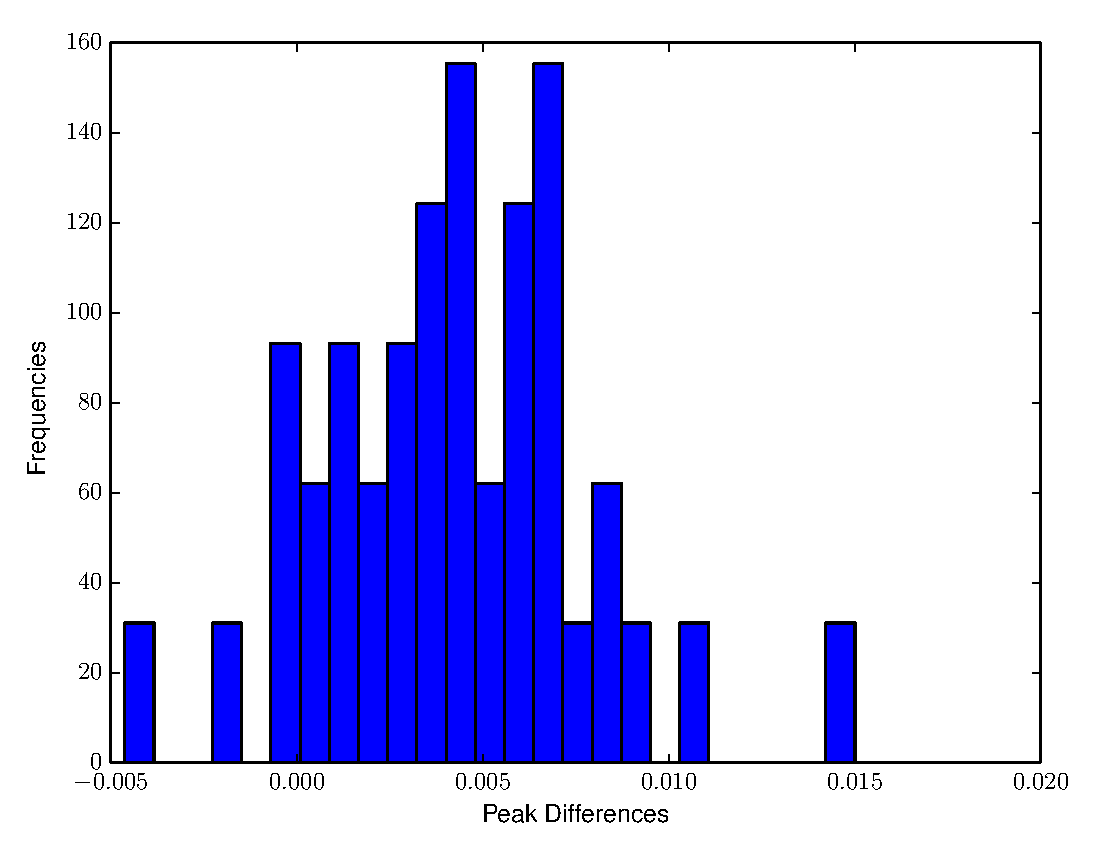
\includegraphics[scale=0.8]{figs/noise_peak_dist.eps}
    \caption{Noise Peak Heights Histogram}
  \end{center}
\end{figure}

\begin{figure}[ht]
  \begin{center}
    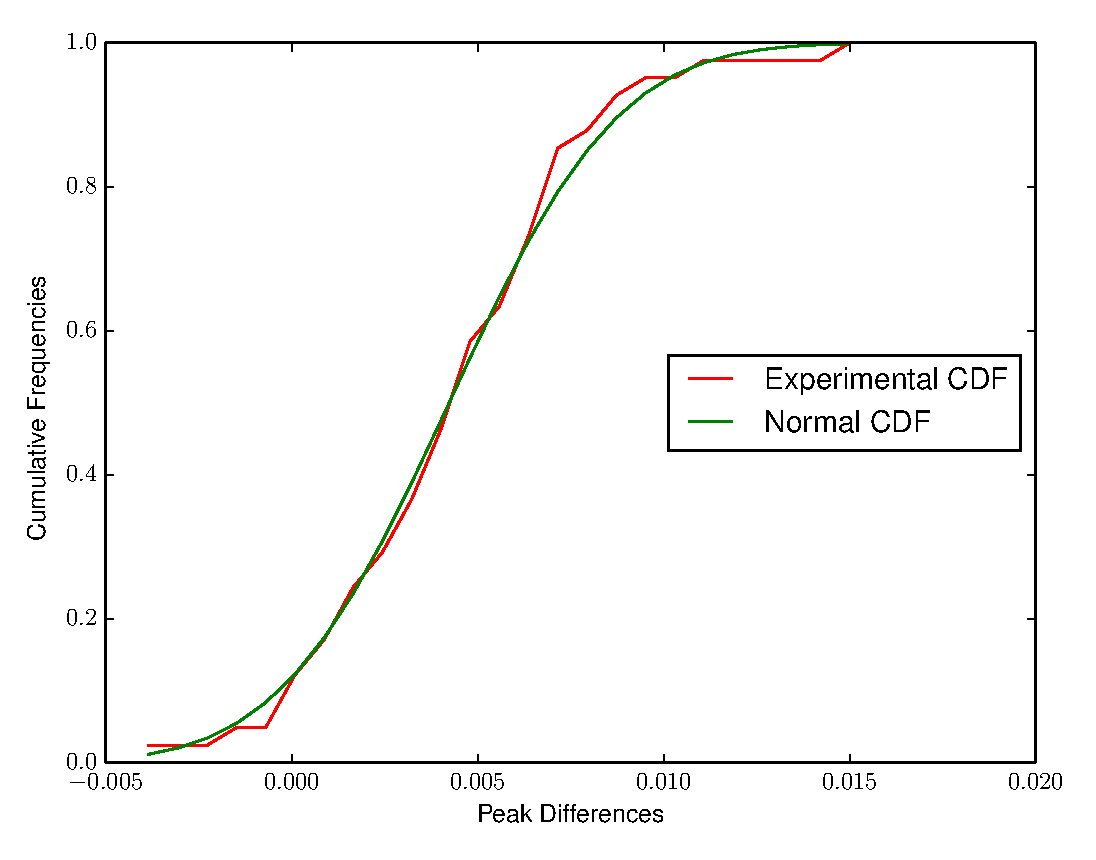
\includegraphics[scale=0.8]{figs/noise_peak_cdf.eps}
    \caption{Noise Peak Heights Distribution}
  \end{center}
\end{figure}
\clearpage

\subsubsection{Sample Noisy Image}
To generate the simulated experimental images, I first sample the number of
peaks, the peak locations, and the peak heights from their respective
distributions. Then this noise is added to the original image and the resulting
image is re-normalized.

\begin{figure}[ht]
  \begin{center}
    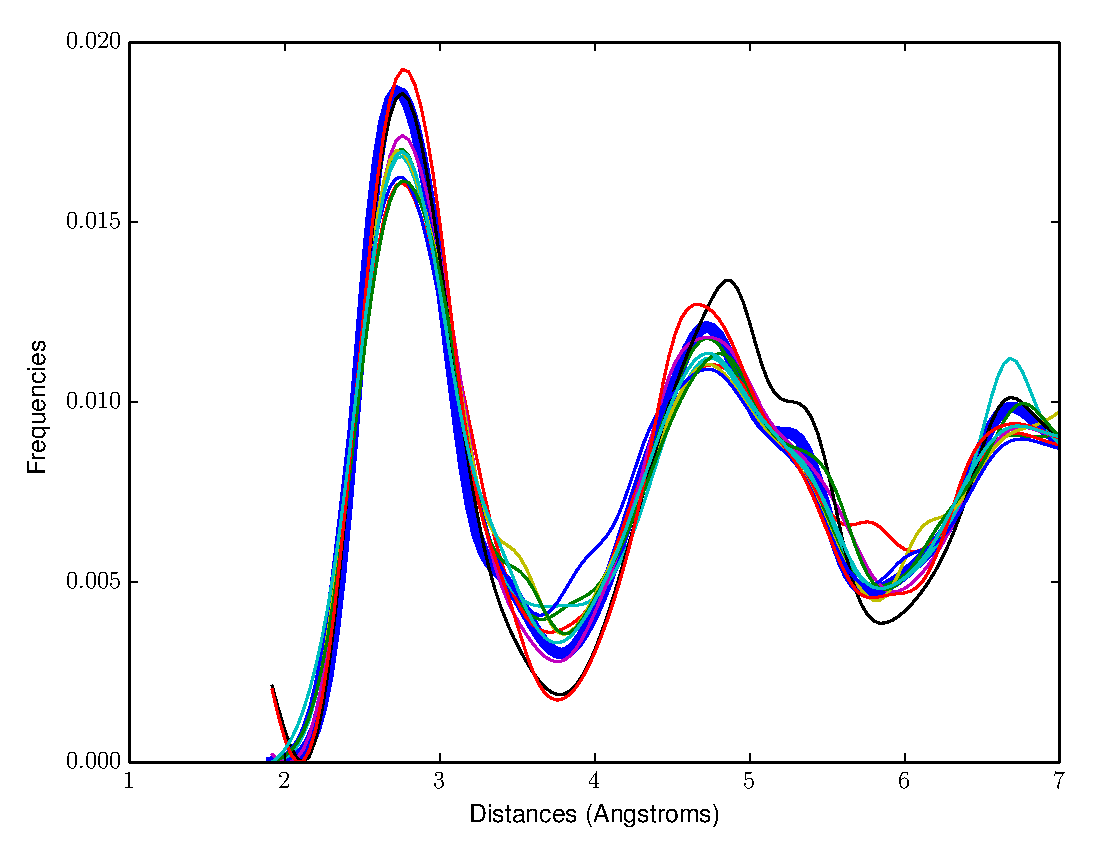
\includegraphics[scale=0.8]{figs/RandomImgs1x.eps}
    \caption{Simulated Experimental Images, 1x Standard Deviation}
  \end{center}
\end{figure}

\begin{figure}[ht]
  \begin{center}
    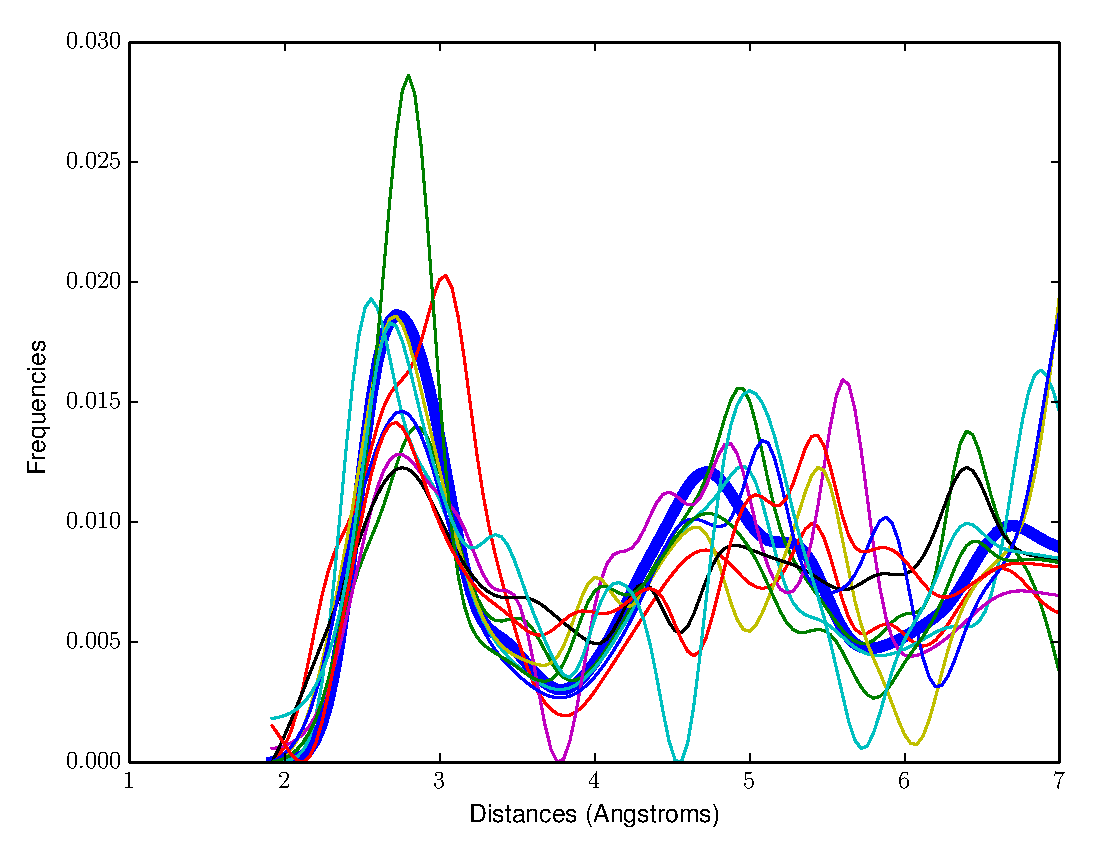
\includegraphics[scale=0.8]{figs/RandomImgs10x.eps}
    \caption{Simulated Experimental Images, 10x Standard Deviation}
  \end{center}
\end{figure}
\clearpage

\section{Recognition Using Eigenfaces}
% experimental accuracy - by pca dim
% synthetic accuracy - by pca dim
\subsection{Mean Image}
\begin{figure}[ht]
  \begin{center}
    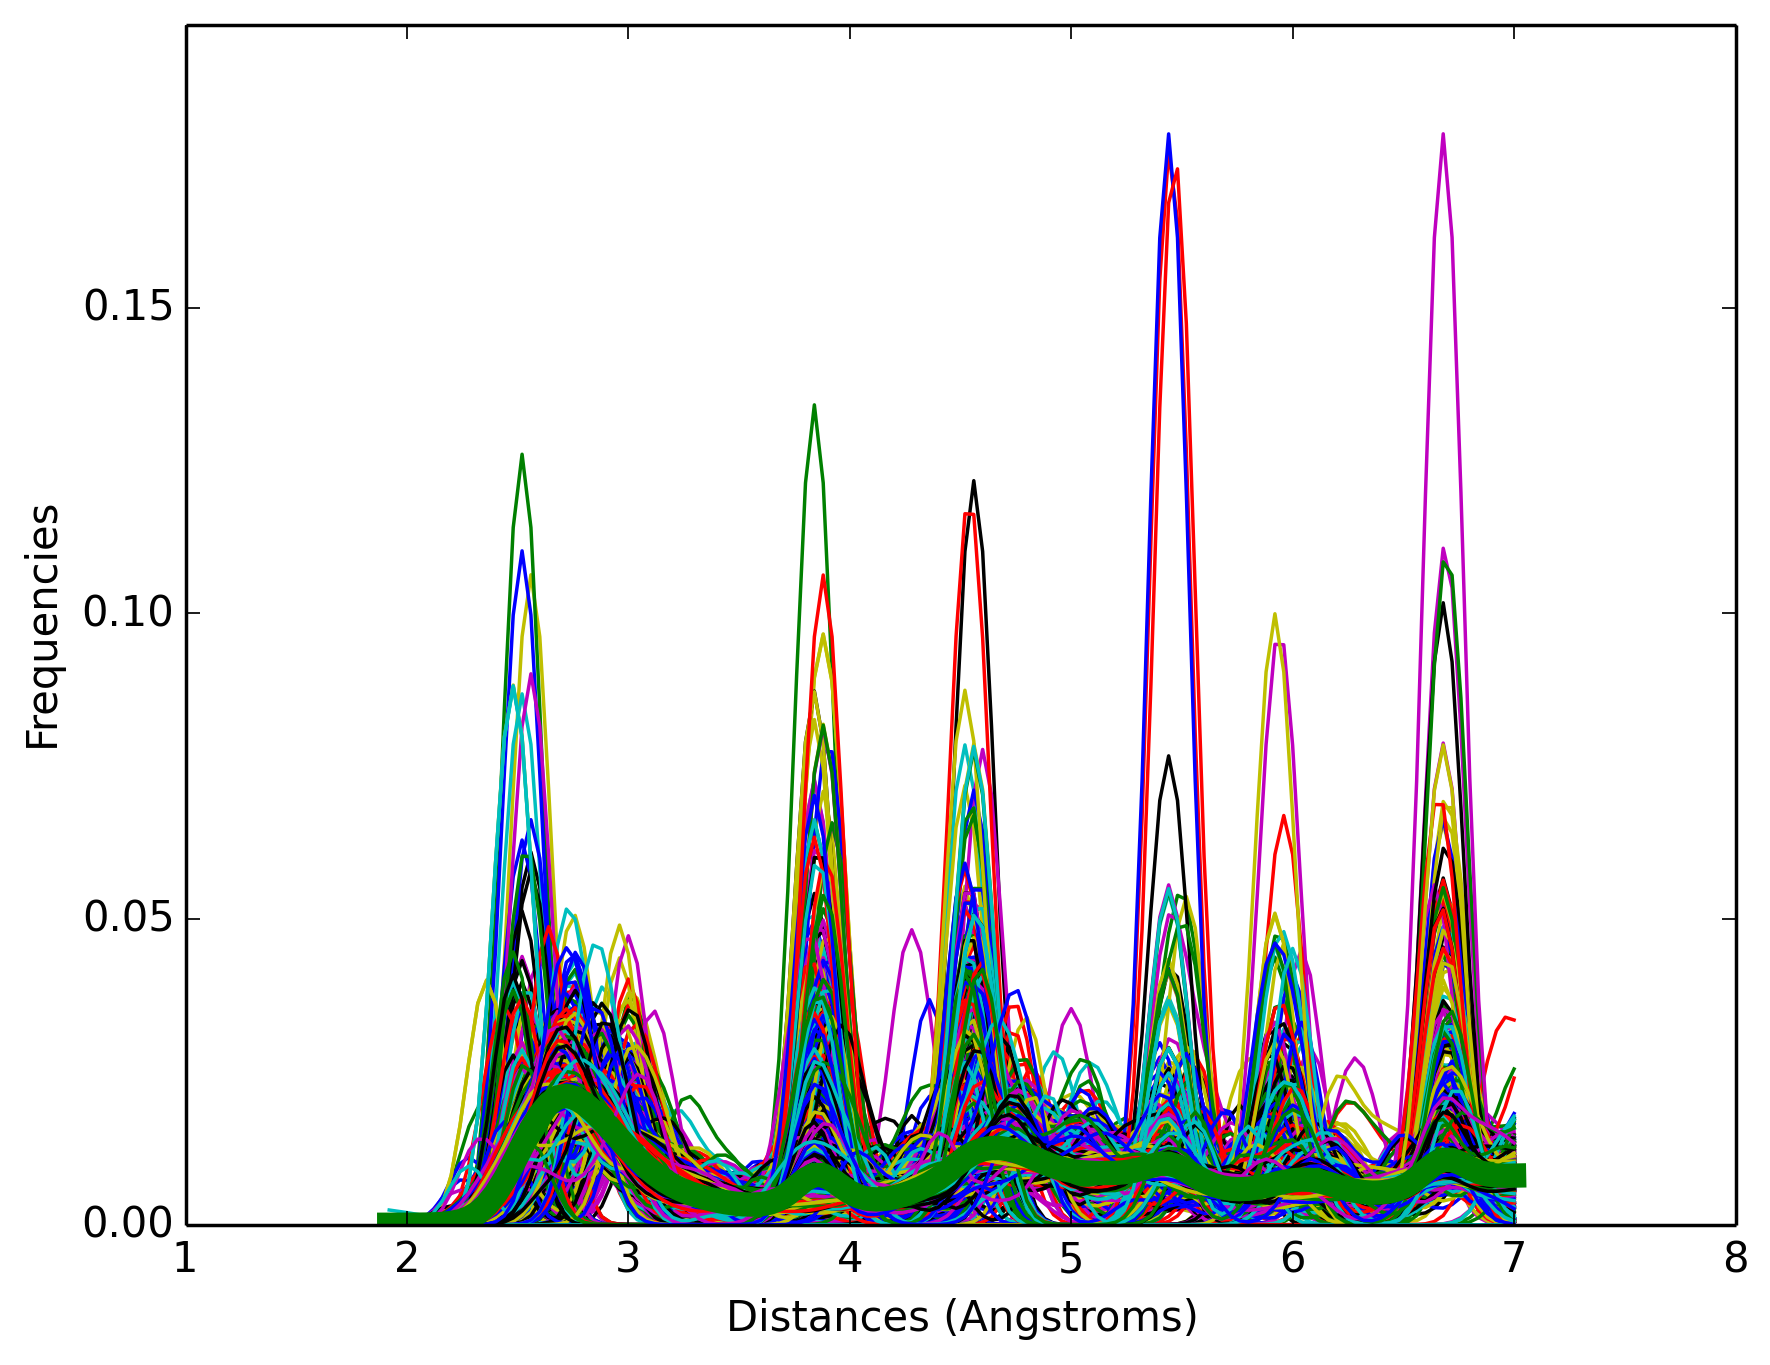
\includegraphics[scale=0.8]{figs/all_calc_images_mean.png}
    \caption{All Calculated Images with Mean}
  \end{center}
\end{figure}
\clearpage

\subsection{Variance Explained by Principal Components}
Principal component analysis projects the data onto an orthogonal space. Thus in
PCA space, we can consider the variance contributed by each of the principal
components separately and can identify those principal components that
contribute most to the variance of the data set. To identify how many principal
components are needed to explain the majority of the variation in the data set,
we can look at the cumulative variance.

\begin{align*}
  C_k = \sum_{i=1}^{k} \sigma_i^2 / \sum_{i=1}^n \sigma_i^2
\end{align*}

where $C_k$ is the variance explained by $k$ principal components and
$\sigma_i^2$ is the variance of principal component $i$.

From the graph, we notice that around 15 principal components explain about 95\%
of the data.

\begin{figure}[ht]
  \begin{center}
    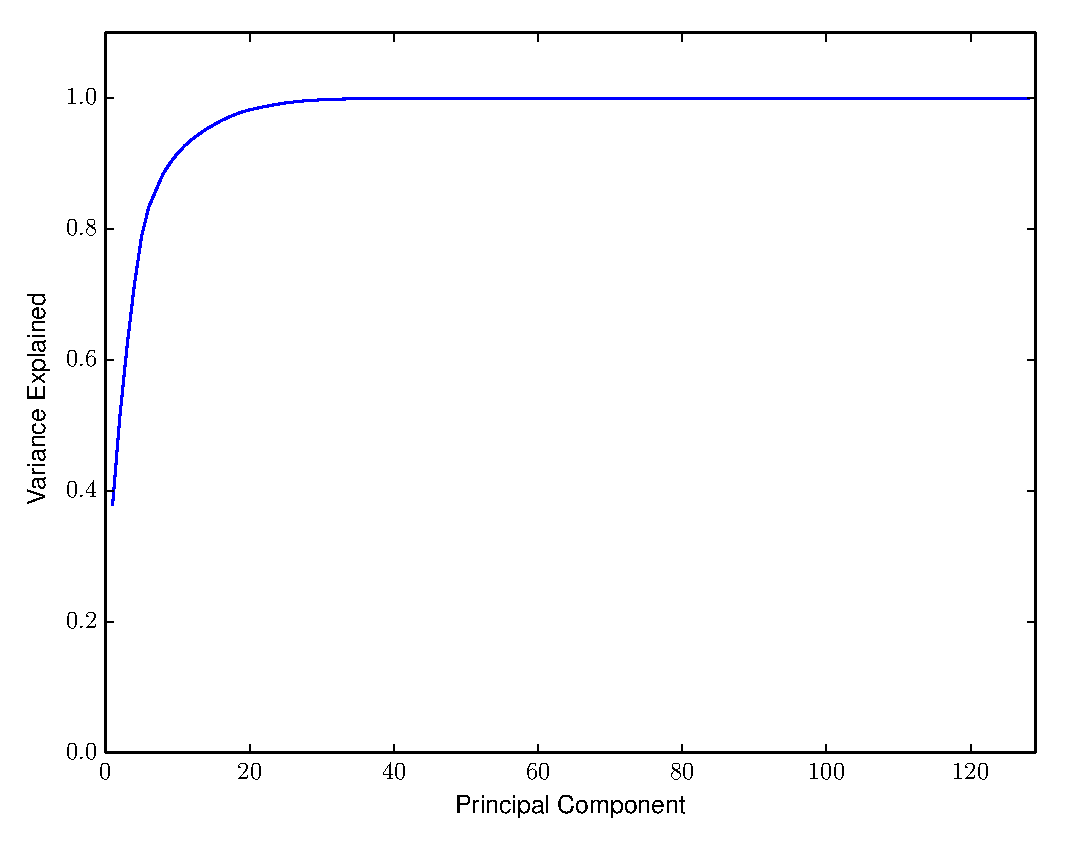
\includegraphics[scale=0.8]{figs/eigenfaces_varexplained.eps}
    \caption{Cumulative Variance Explained by Principal Components}
  \end{center}
\end{figure}
\clearpage

% TODO: need to rerun the results with the new smoothing coefficient.
\subsection{Eigenfaces}
!!! Need to rerun all of these results with the changed smoothing coefficient!!!
Here, we plot the eigenfaces to see if any key features of the images are
revealed. Not much of anything is noteworthy.

\begin{figure}[ht]
  \begin{center}
    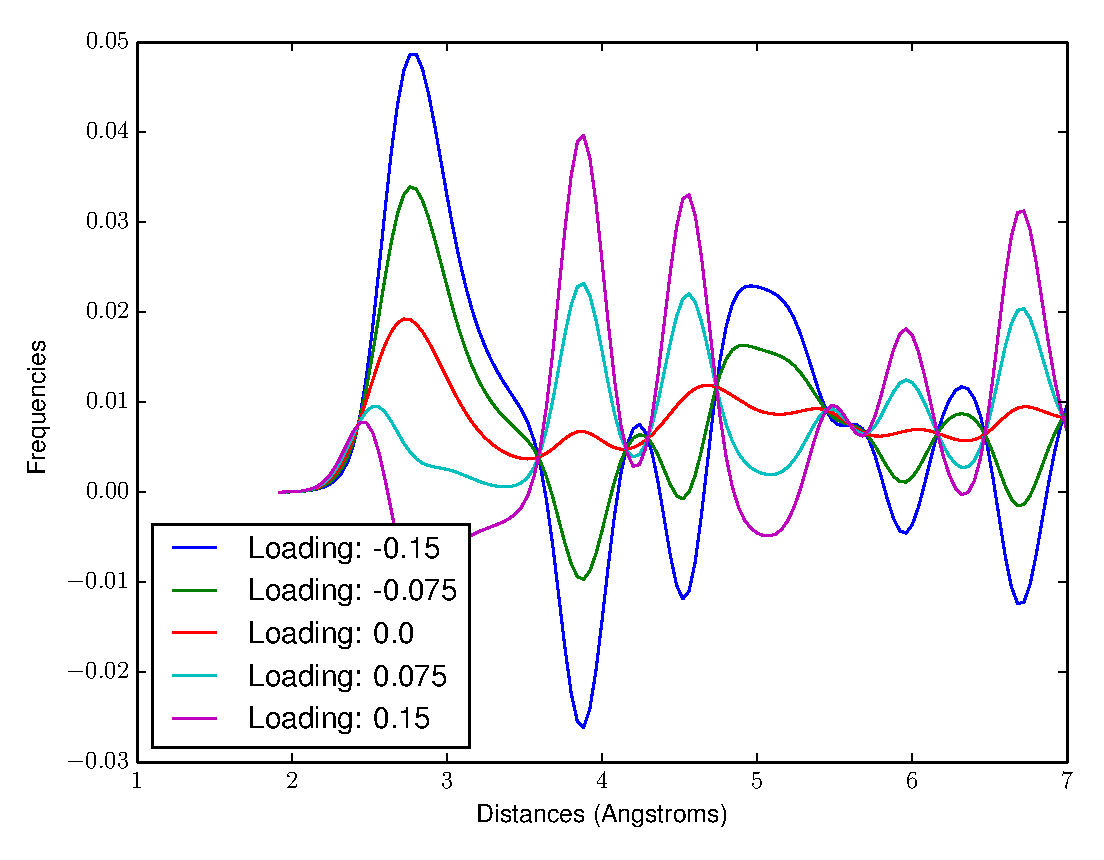
\includegraphics[scale=0.8]{figs/eigenface1.eps}
    \caption{First Eigenface}
  \end{center}
\end{figure}

\begin{figure}[ht]
  \begin{center}
    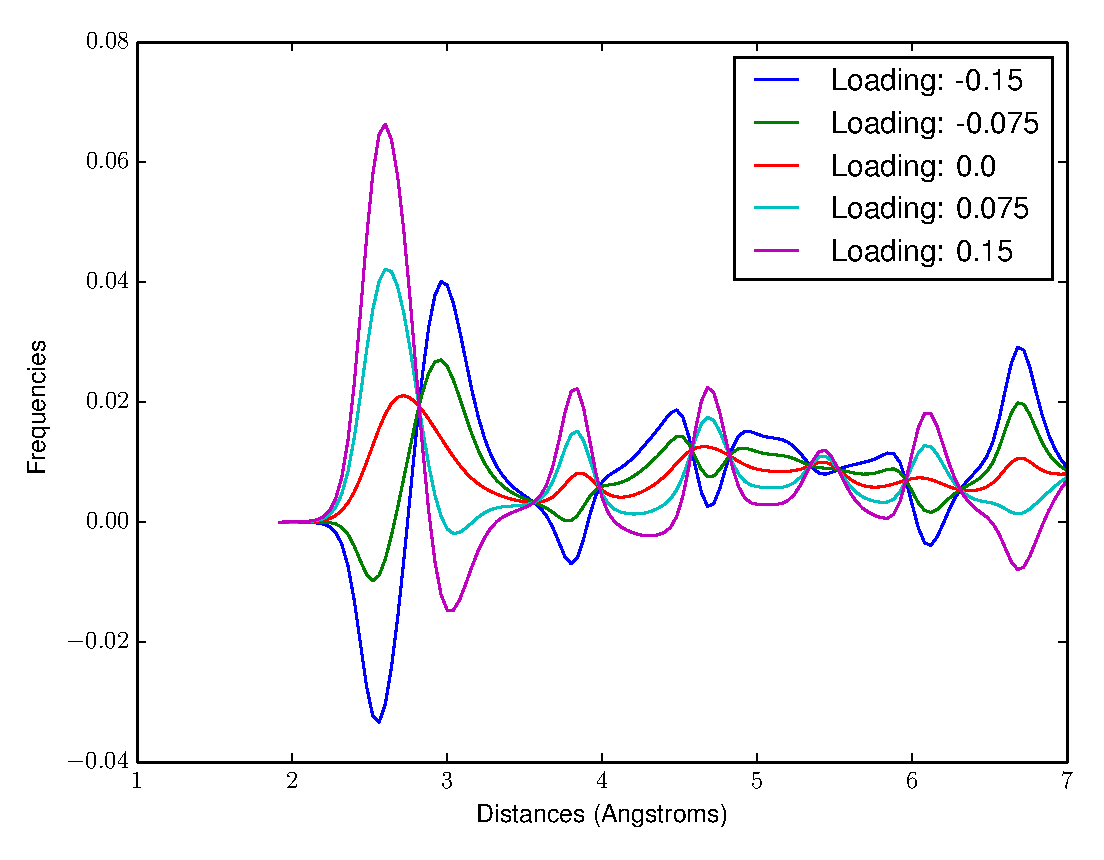
\includegraphics[scale=0.8]{figs/eigenface2.eps}
    \caption{Second Eigenface}
  \end{center}
\end{figure}

\begin{figure}[ht]
  \begin{center}
    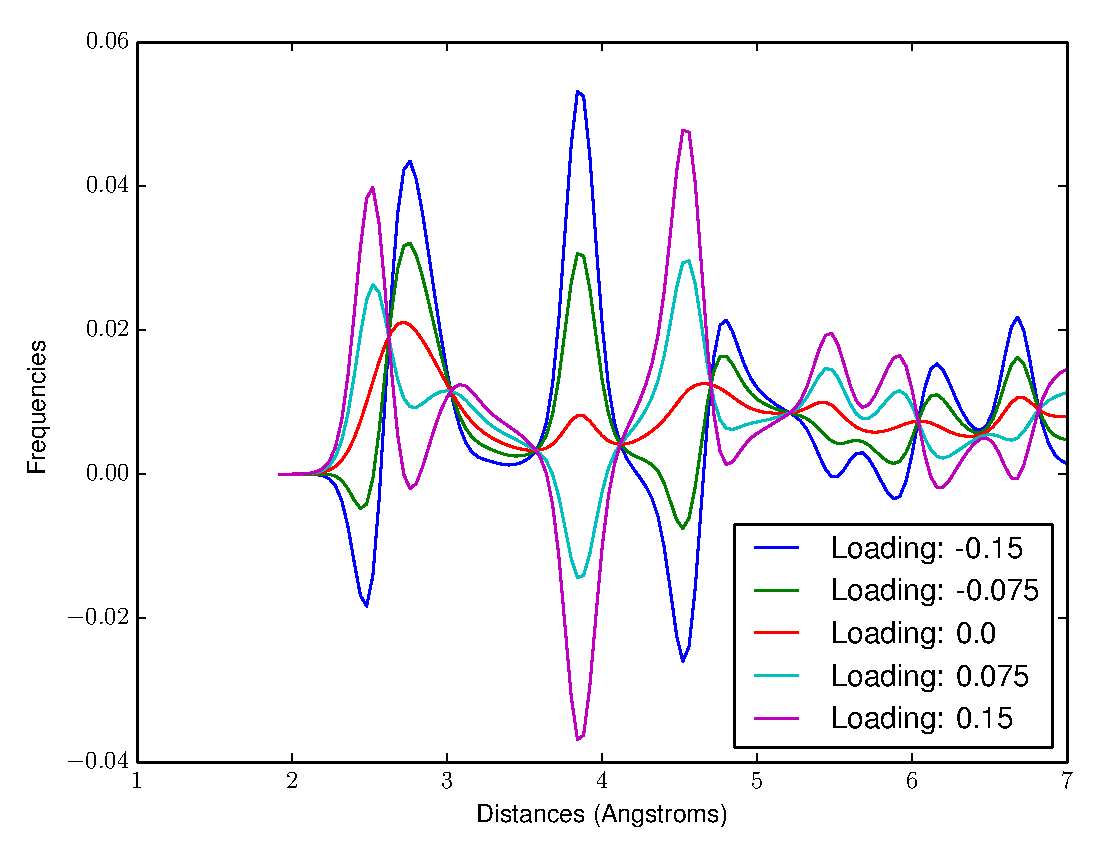
\includegraphics[scale=0.8]{figs/eigenface3.eps}
    \caption{Third Eigenface}
  \end{center}
\end{figure}
\clearpage

\subsection{Data in Eigenspace}
Below shows the data in principal component space for the most significant
principal components.

One feature we observe is that the first principal component separates the
experiemental data very well and in fact appropriately sorts the silicon lithium
structures by that amount of lithium. Higher principal components are useful for
distinguishing the experimental images.

\begin{figure}[ht]
  \begin{center}
    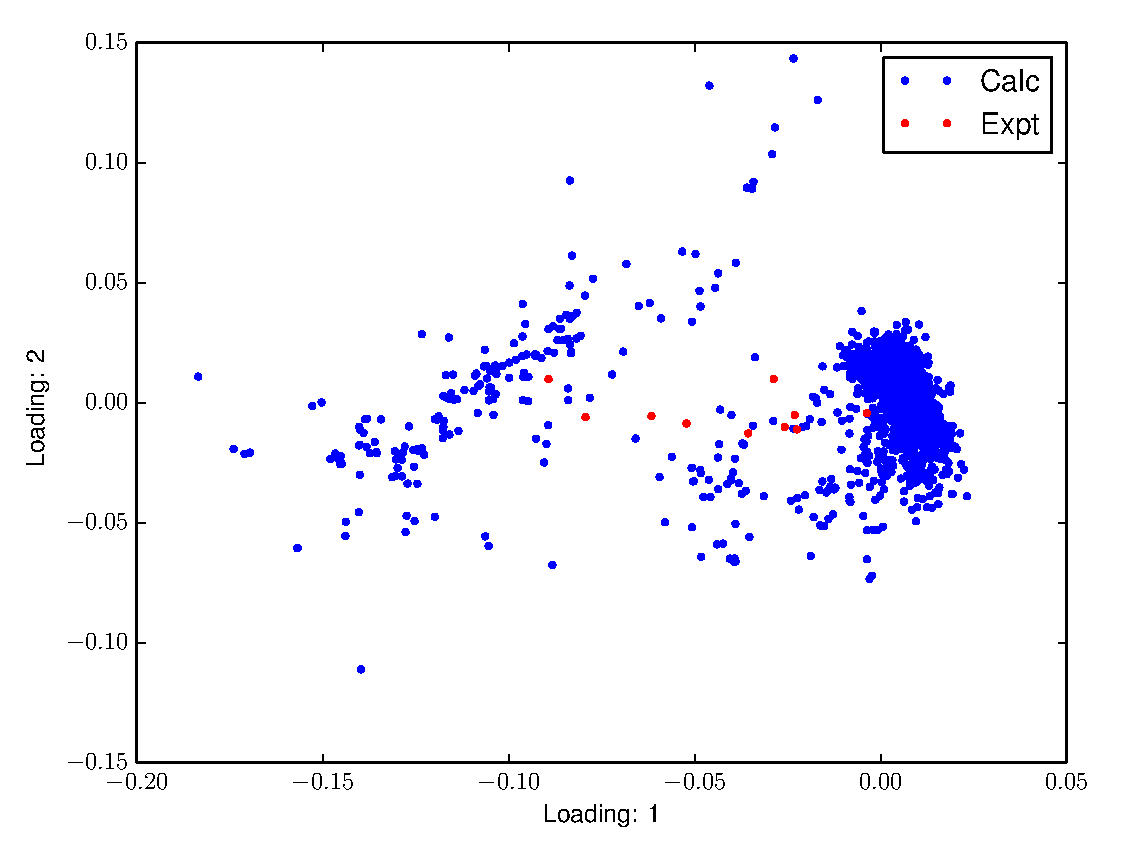
\includegraphics[scale=0.8]{figs/eigenspace1-2.eps}
    \caption{Loading 1 vs  Loading 2}
  \end{center}
\end{figure}

\begin{table}[ht]
  \begin{center}
  \begin{tabular}{|l|l|l|}
    \hline
    \textbf{Label} & \textbf{Loading 1} & \textbf{Loading 2} \\ \hline
    SiLiExpt1      & -0.0893            & 0.00982            \\ \hline
    SiLiExpt2      & -0.0794            & -0.006             \\ \hline
    SiLiExpt3      & -0.0616            & -0.0055            \\ \hline
    SiLiExpt4      & -0.0522            & -0.0086            \\ \hline
    SiLiExpt5      & -0.0356            & -0.0128            \\ \hline
    ExptGaAs       & -0.0288            & 0.00994            \\ \hline
    SiLiExpt7      & -0.0258            & -0.0101            \\ \hline
    SiLiExpt6      & -0.0231            & -0.0051            \\ \hline
    SiLiExpt8      & -0.0226            & -0.0111            \\ \hline
    ExptInAs       & -0.0038            & -0.0044            \\ \hline
  \end{tabular}
  \caption{Experimental Data Sorted by Loading 1}
  \end{center}
\end{table}

\begin{table}[h]
  \begin{center}
  \begin{tabular}{|l|l|l|}
    \hline
    \textbf{Label} & \textbf{Loading 1} & \textbf{Loading 2} \\ \hline
    SiLiExpt5      & -0.0356            & -0.0128            \\ \hline
    SiLiExpt8      & -0.0226            & -0.0111            \\ \hline
    SiLiExpt7      & -0.0258            & -0.0101            \\ \hline
    SiLiExpt4      & -0.0522            & -0.0086            \\ \hline
    SiLiExpt2      & -0.0794            & -0.006             \\ \hline
    SiLiExpt3      & -0.0616            & -0.0055            \\ \hline
    SiLiExpt6      & -0.0231            & -0.0051            \\ \hline
    ExptInAs       & -0.0038            & -0.0044            \\ \hline
    SiLiExpt1      & -0.0893            & 0.00982            \\ \hline
    ExptGaAs       & -0.0288            & 0.00994            \\ \hline
  \end{tabular}
  \caption{Experimental Data Sorted by Loading 2}
  \end{center}
\end{table}

\begin{figure}[ht]
  \begin{center}
    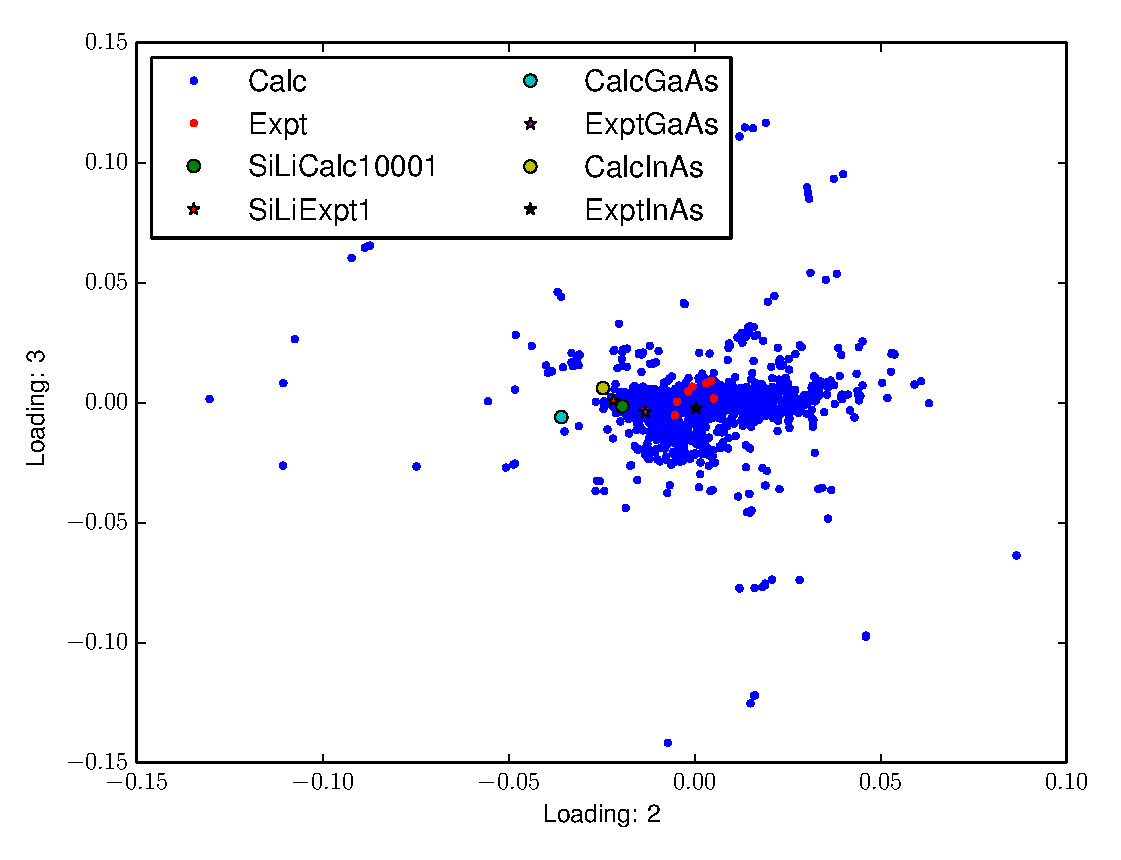
\includegraphics[scale=0.8]{figs/eigenspace2-3.eps}
    \caption{Loading 2 vs  Loading 3}
  \end{center}
\end{figure}

\begin{figure}[ht]
  \begin{center}
    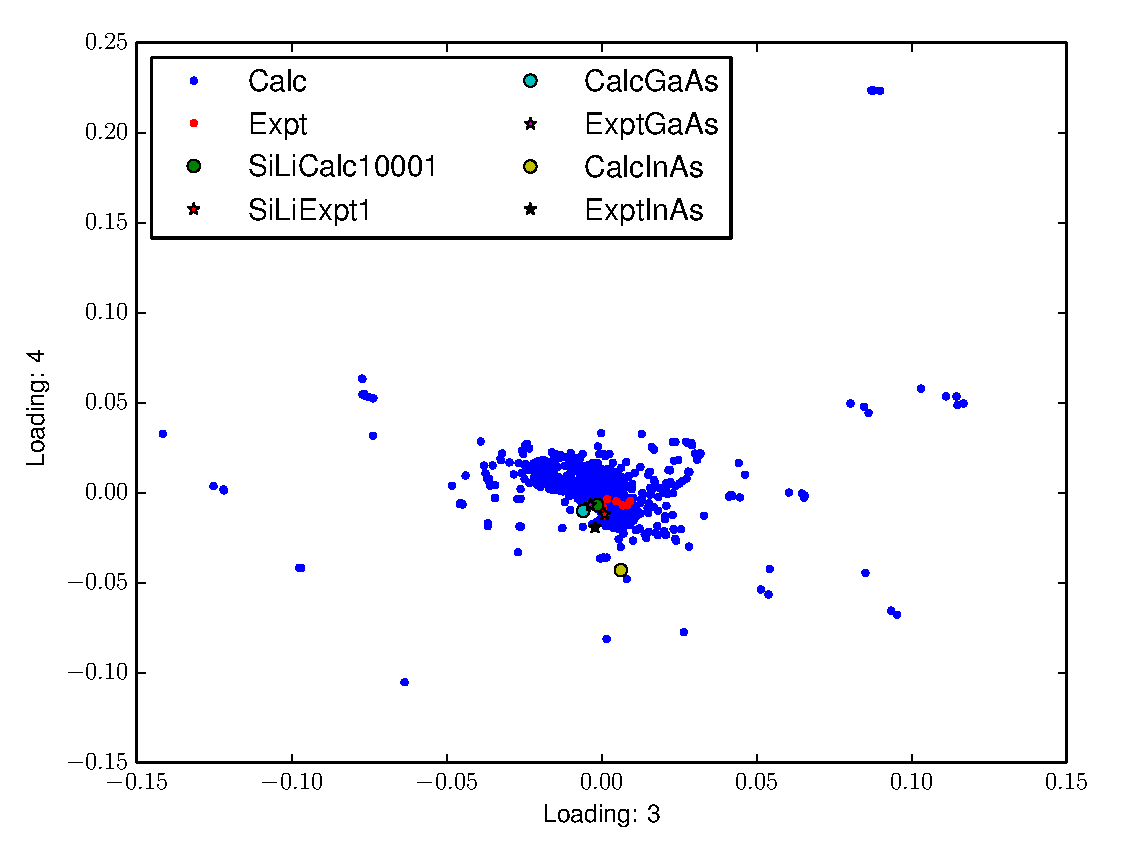
\includegraphics[scale=0.8]{figs/eigenspace3-4.eps}
    \caption{Loading 3 vs  Loading 4}
  \end{center}
\end{figure}

\begin{figure}[ht]
  \begin{center}
    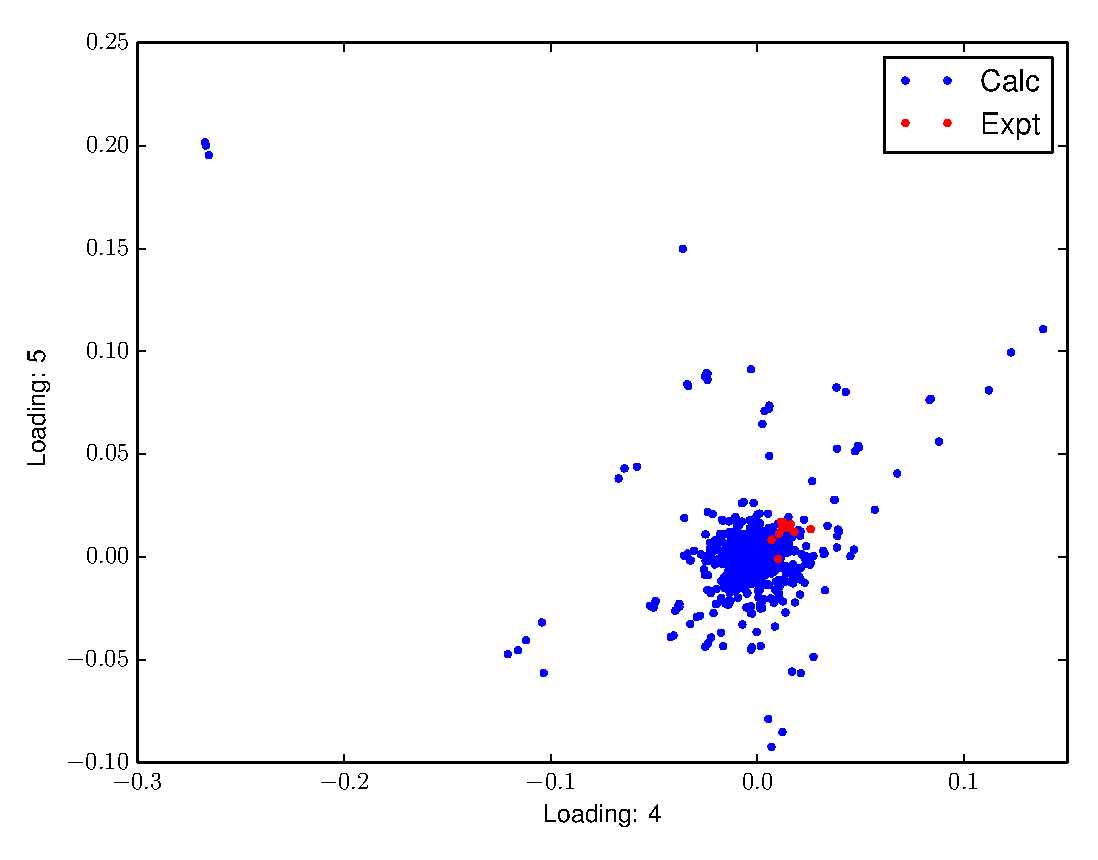
\includegraphics[scale=0.8]{figs/eigenspace4-5.eps}
    \caption{Loading 4 vs  Loading 5}
  \end{center}
\end{figure}
\clearpage

\subsubsection{Eigenspace Outliers}
Given that the higher order principal components did not separate the
experimental images, we looked at the images with high loading values. 

From the plots below, we notice that the higher order principal components
capture the very high peaks in images. Indeed for some images that have very few
peaks, after normalization those peaks will become much higher than those images
that have many peaks.

\begin{figure}[ht]
  \begin{center}
    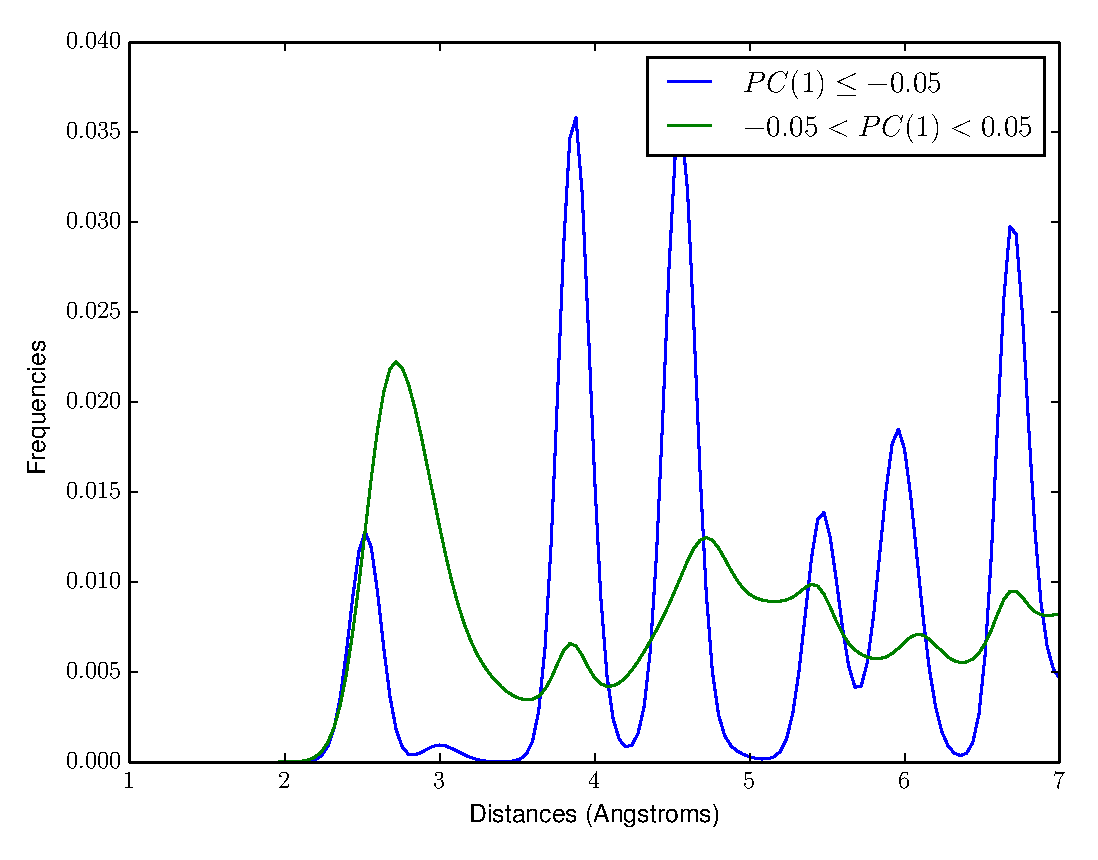
\includegraphics[scale=0.8]{figs/eigenOutlier1.eps}
    \caption{First Principal Component Outliers}
  \end{center}
\end{figure}

\begin{figure}[ht]
  \begin{center}
    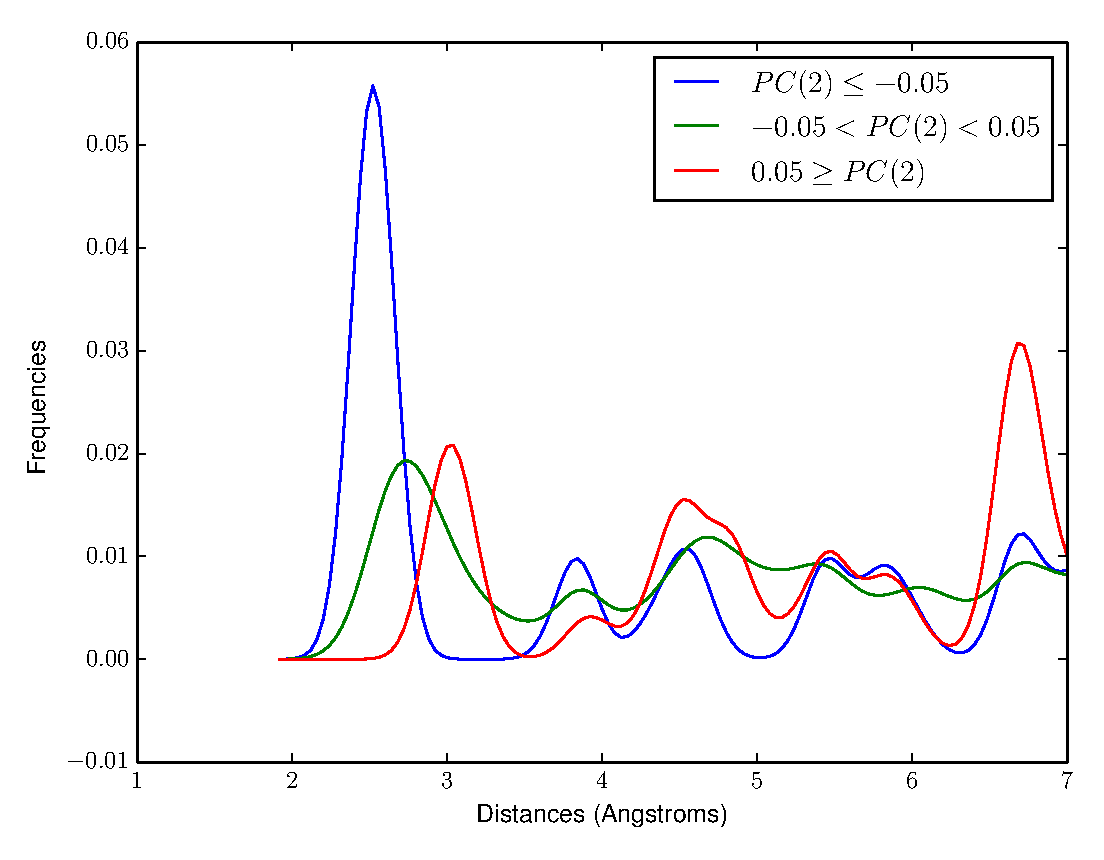
\includegraphics[scale=0.8]{figs/eigenOutlier2.eps}
    \caption{Second Principal Component Outliers}
  \end{center}
\end{figure}

\begin{figure}[ht]
  \begin{center}
    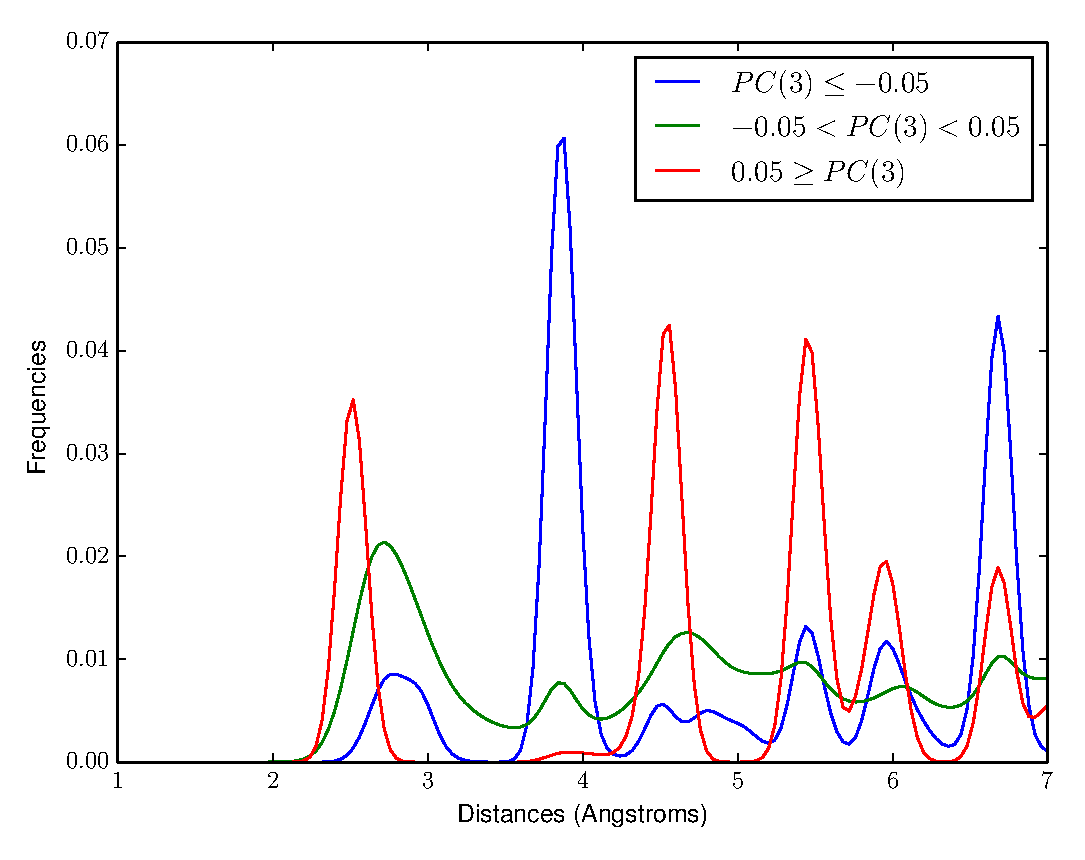
\includegraphics[scale=0.8]{figs/eigenOutlier3.eps}
    \caption{Third Principal Component Outliers}
  \end{center}
\end{figure}

\begin{figure}[ht]
  \begin{center}
    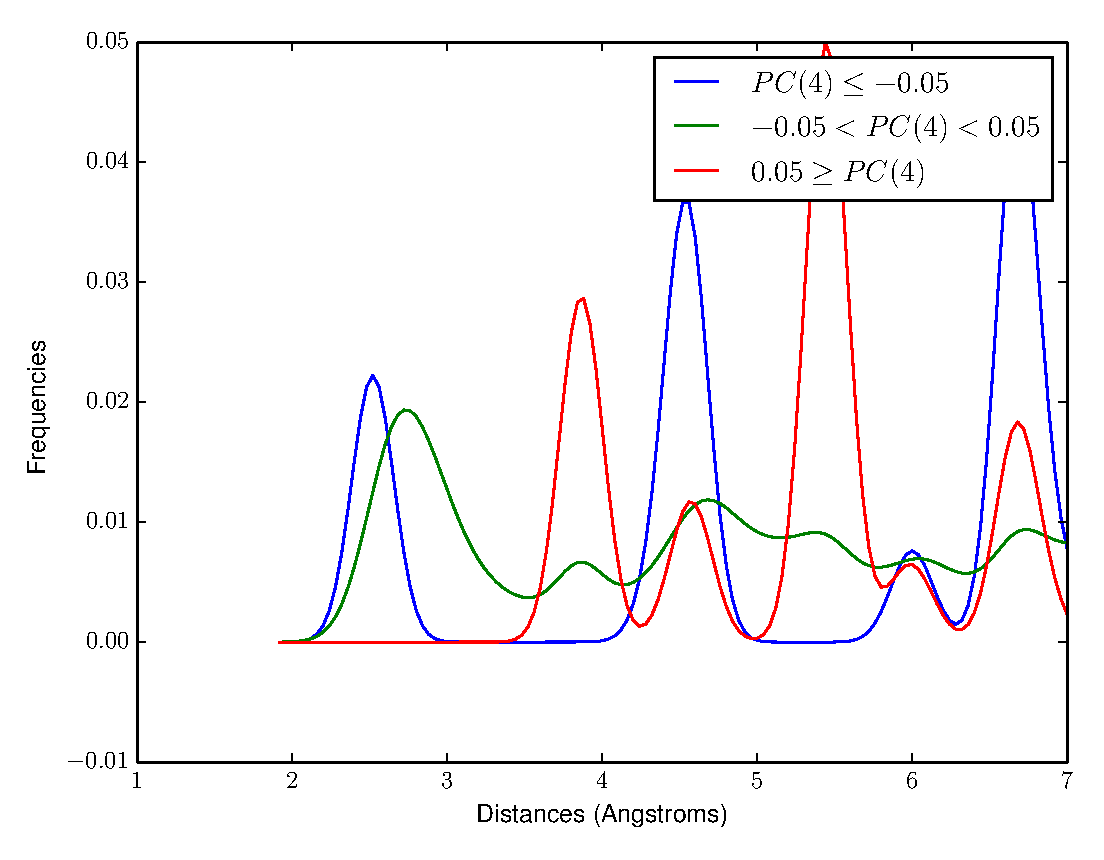
\includegraphics[scale=0.8]{figs/eigenOutlier4.eps}
    \caption{Fourth Principal Component Outliers}
  \end{center}
\end{figure}

\begin{figure}[ht]
  \begin{center}
    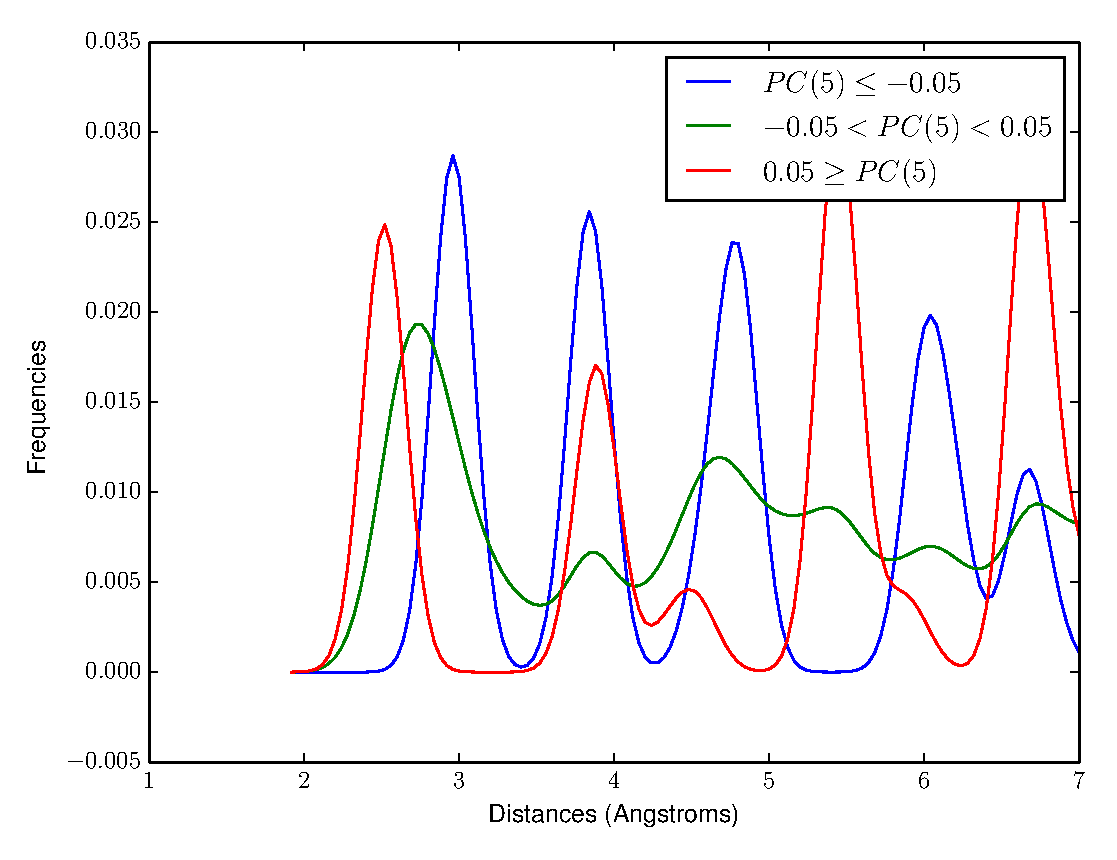
\includegraphics[scale=0.8]{figs/eigenOutlier5.eps}
    \caption{Fifth Principal Component Outliers}
  \end{center}
\end{figure}
\clearpage

\subsection{Experimental Image Recognition}
Here we compute the best matches in PCA space for the experimental images for
the first 3, 10, and all principal components.
\subsubsection{3 Principal Components}
\begin{table}[h]
  \begin{center}
\begin{tabular}{|l|l|l|l|l|l|}
\hline
\textbf{Image}     & \textbf{Best Match} & \textbf{2}    & \textbf{3}    & \textbf{4}    & \textbf{5}    \\ \hline
\textbf{ExptGaAs}  & SiLiCalc11436       & SiLiCalc11634 & SiLiCalc11967 & SiLiCalc12738 & SiLiCalc10225 \\ \hline
\textbf{ExptInAs}  & SiLiCalc10643       & SiLiCalc10560 & SiLiCalc10693 & SiLiCalc10617 & SiLiCalc10621 \\ \hline
\textbf{SiLiExpt1} & SiLiCalc10208       & SiLiCalc10315 & SiLiCalc10317 & SiLiCalc10188 & SiLiCalc10187 \\ \hline
\textbf{SiLiExpt2} & SiLiCalc10317       & SiLiCalc10287 & SiLiCalc10320 & SiLiCalc10283 & SiLiCalc10273 \\ \hline
\textbf{SiLiExpt3} & SiLiCalc10287       & SiLiCalc10239 & SiLiCalc10259 & SiLiCalc10317 & SiLiCalc10232 \\ \hline
\textbf{SiLiExpt4} & SiLiCalc10229       & SiLiCalc10225 & SiLiCalc10232 & SiLiCalc10239 & SiLiCalc10259 \\ \hline
\textbf{SiLiExpt5} & SiLiCalc10225       & SiLiCalc10256 & SiLiCalc10232 & SiLiCalc10229 & SiLiCalc10231 \\ \hline
\textbf{SiLiExpt6} & SiLiCalc10322       & SiLiCalc10225 & SiLiCalc10247 & SiLiCalc10229 & SiLiCalc10256 \\ \hline
\textbf{SiLiExpt7} & SiLiCalc10225       & SiLiCalc10322 & SiLiCalc10256 & SiLiCalc10247 & SiLiCalc10229 \\ \hline
\textbf{SiLiExpt8} & SiLiCalc10225       & SiLiCalc10322 & SiLiCalc10247 & SiLiCalc10337 & SiLiCalc10256 \\ \hline
\end{tabular}
  \caption{Recognition with 3 Principal Components}
  \end{center}
\end{table}

\begin{figure}[ht]
  \begin{center}
    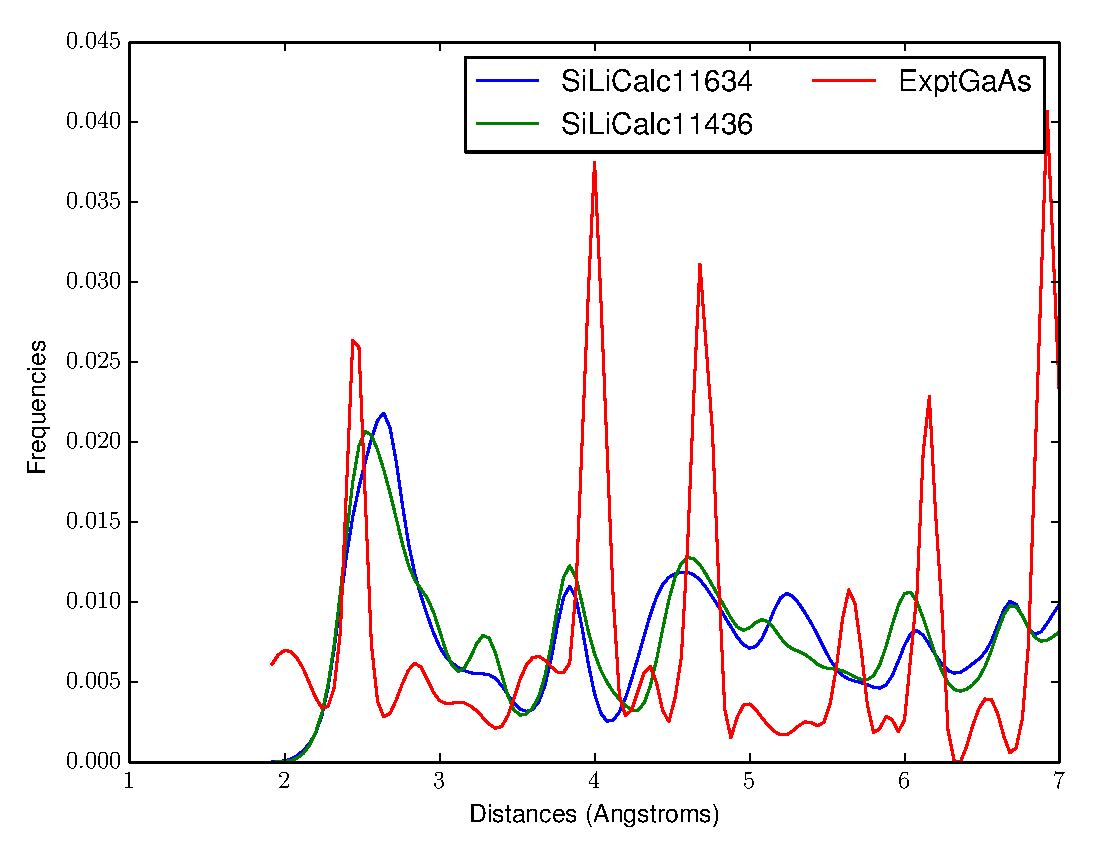
\includegraphics[scale=0.8]{figs/PC3MatchExptGaAs-SiLiCalc11436-SiLiCalc11634.eps}
  \caption{PCA Matches: ExptGaAs, SiLiCalc11436, SiLiCalc11634}
  \end{center}
\end{figure}

\begin{figure}[ht]
  \begin{center}
    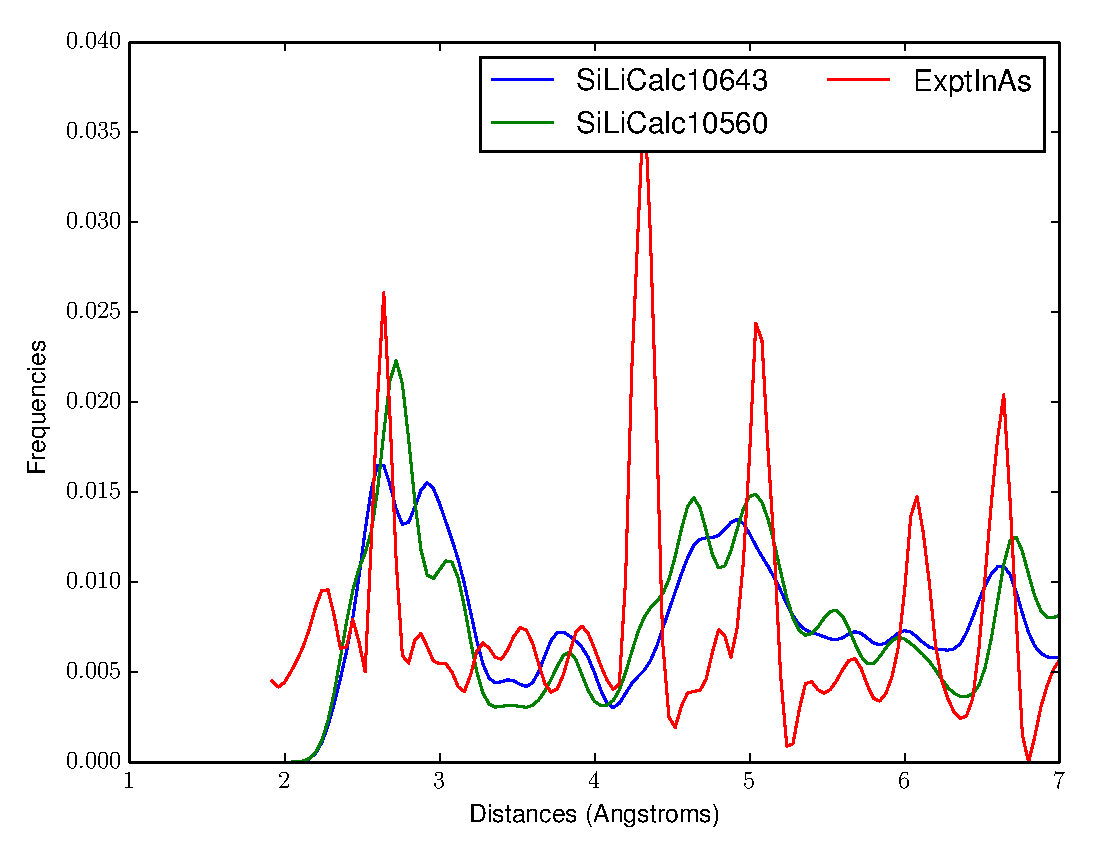
\includegraphics[scale=0.8]{figs/PC3MatchExptInAs-SiLiCalc10643-SiLiCalc10560.eps}
  \caption{PCA Matches: ExptInAs, SiLiCalc10643, SiLiCalc10560}
  \end{center}
\end{figure}

\begin{figure}[ht]
  \begin{center}
    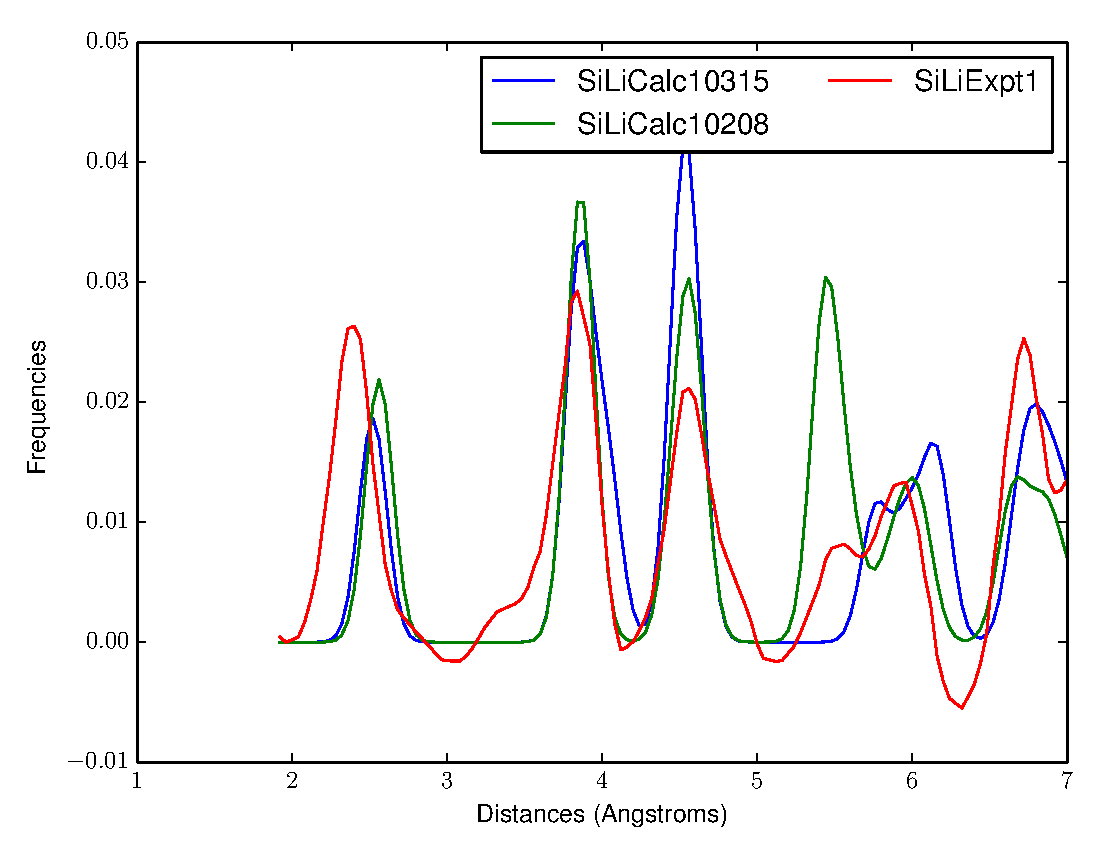
\includegraphics[scale=0.8]{figs/PC3MatchSiLiExpt1-SiLiCalc10208-SiLiCalc10315.eps}
  \caption{PCA Matches: SiLiExpt1, SiLiCalc10208, SiLiCalc10315}
  \end{center}
\end{figure}

\begin{figure}[ht]
  \begin{center}
    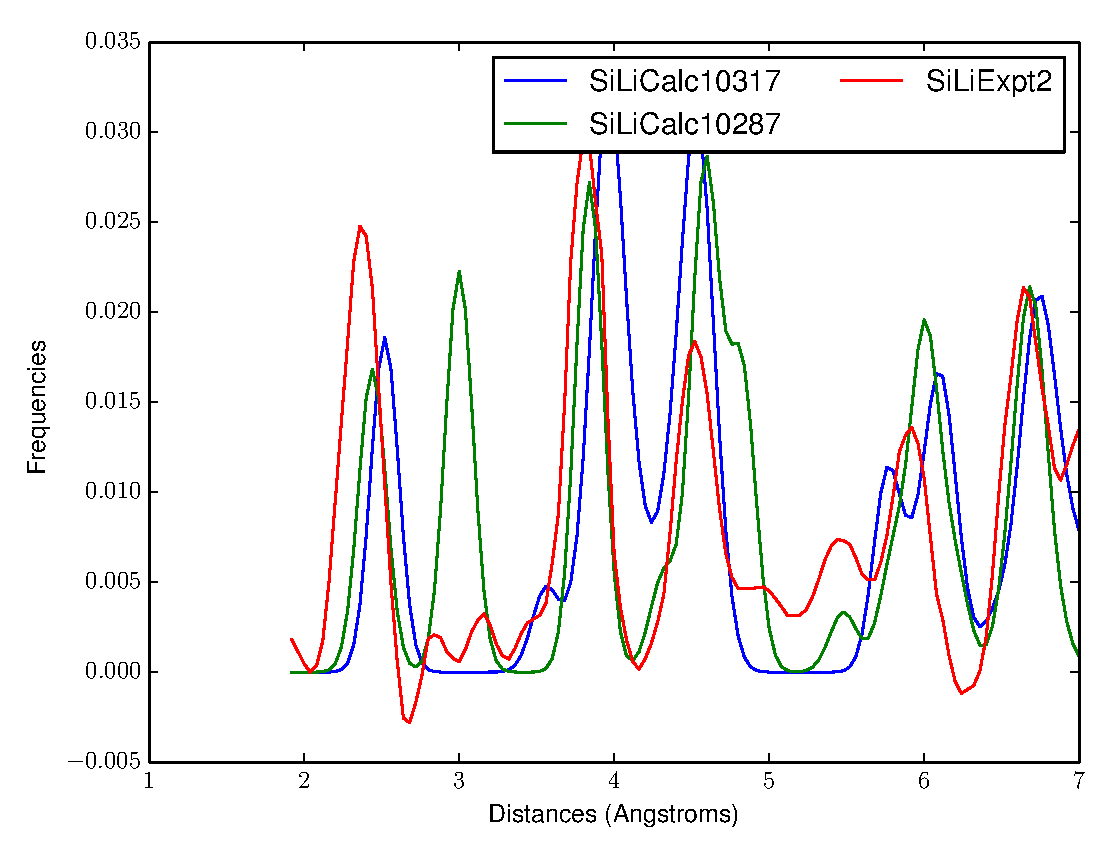
\includegraphics[scale=0.8]{figs/PC3MatchSiLiExpt2-SiLiCalc10317-SiLiCalc10287.eps}
    \caption{PCA Matches: SiLiExpt2, SiLiCalc10317, SiLiCalc10287}
  \end{center}
\end{figure}

\begin{figure}[ht]
  \begin{center}
    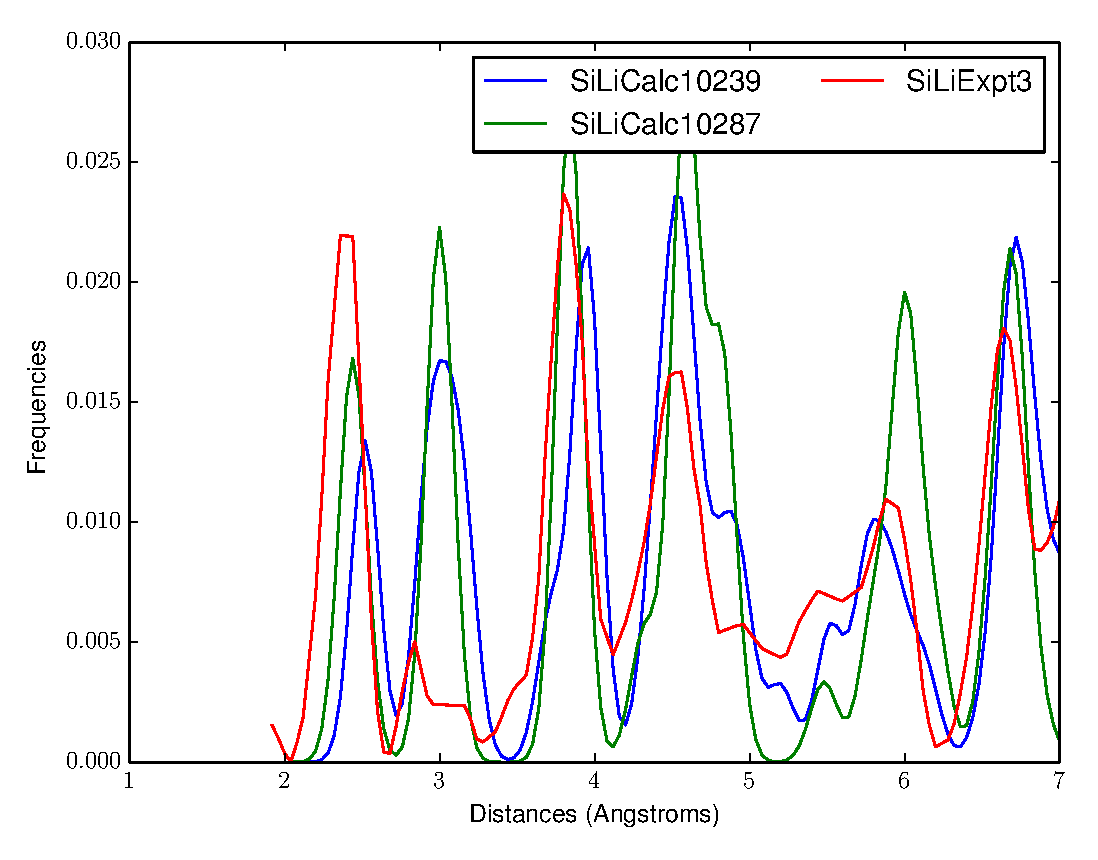
\includegraphics[scale=0.8]{figs/PC3MatchSiLiExpt3-SiLiCalc10287-SiLiCalc10239.eps}
    \caption{PCA Matches: SiLiExpt3, SiLiCalc10287, SiLiCalc10239}
  \end{center}
\end{figure}

\begin{figure}[ht]
  \begin{center}
    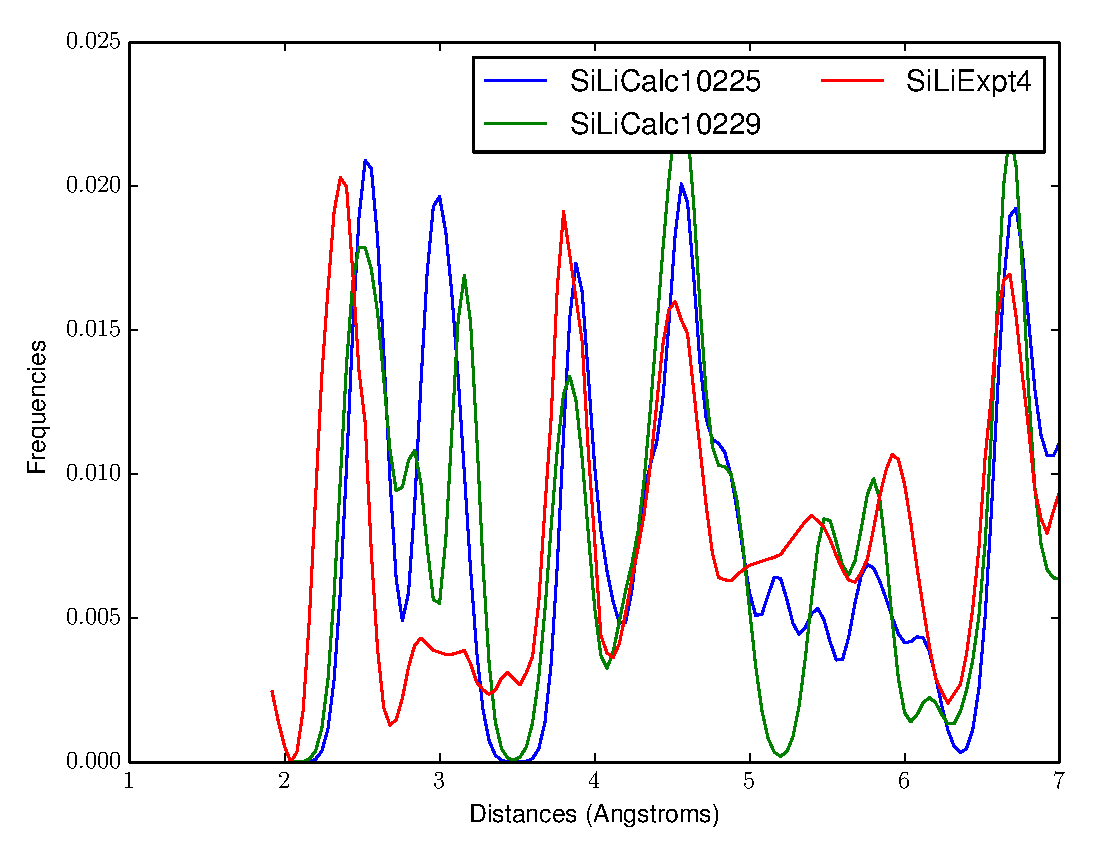
\includegraphics[scale=0.8]{figs/PC3MatchSiLiExpt4-SiLiCalc10229-SiLiCalc10225.eps}
    \caption{PCA Matches: SiLiExpt4, SiLiCalc10229, SiLiCalc10225}
  \end{center}
\end{figure}

\begin{figure}[ht]
  \begin{center}
    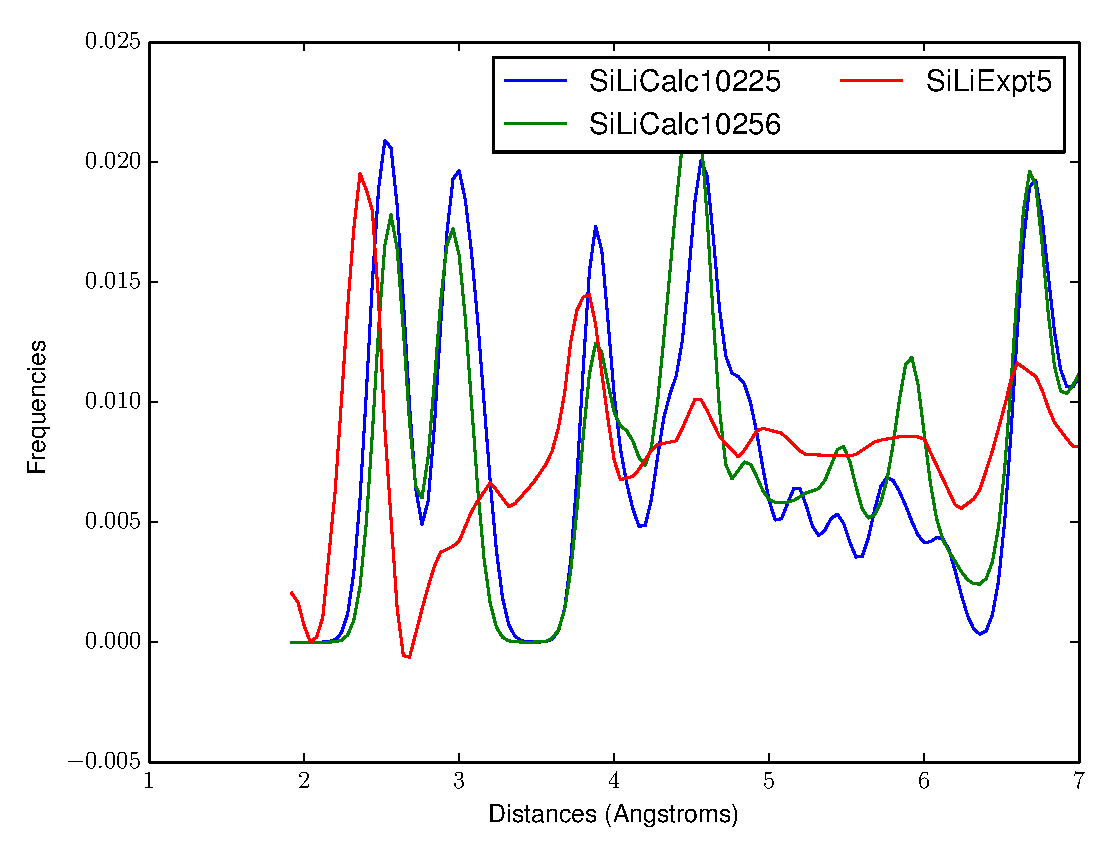
\includegraphics[scale=0.8]{figs/PC3MatchSiLiExpt5-SiLiCalc10225-SiLiCalc10256.eps}
    \caption{PCA Matches: SiLiExpt5, SiLiCalc10225, SiLiCalc10256}
  \end{center}
\end{figure}

\begin{figure}[ht]
  \begin{center}
    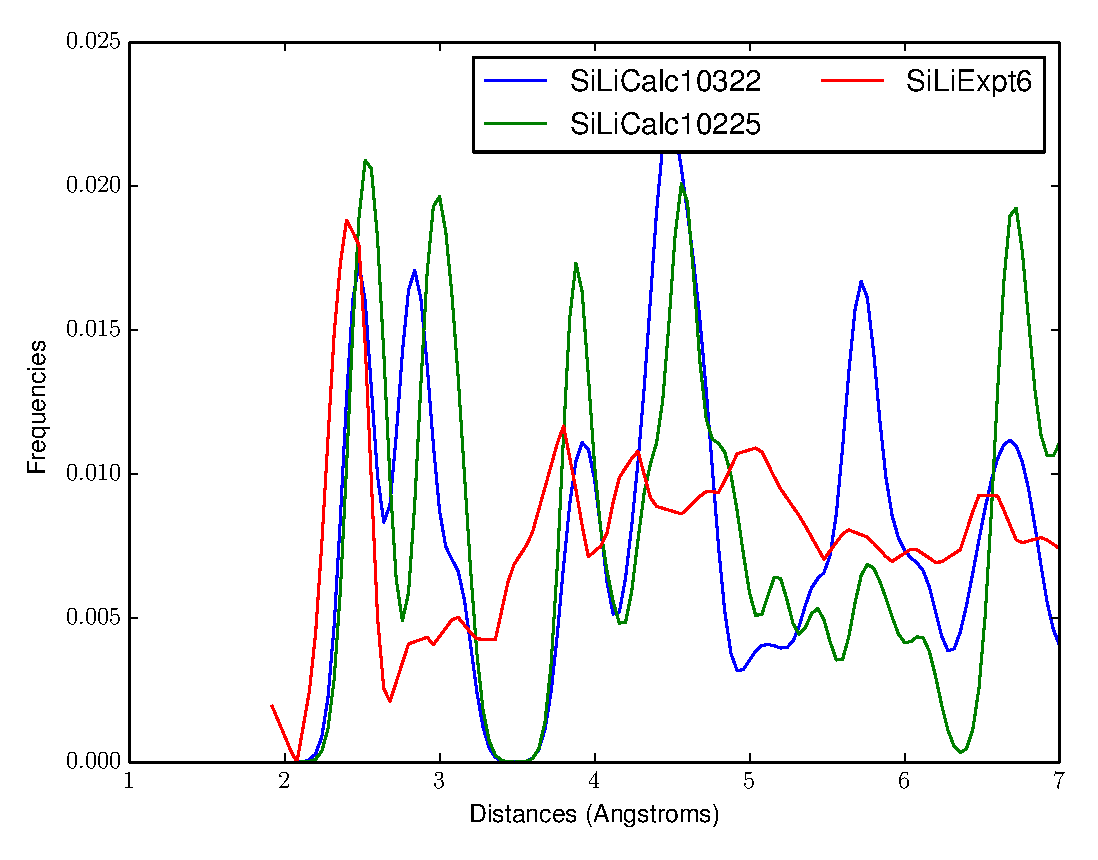
\includegraphics[scale=0.8]{figs/PC3MatchSiLiExpt6-SiLiCalc10322-SiLiCalc10225.eps}
    \caption{PCA Matches: SiLiExpt6, SiLiCalc10322, SiLiCalc10225}
  \end{center}
\end{figure}

\begin{figure}[ht]
  \begin{center}
    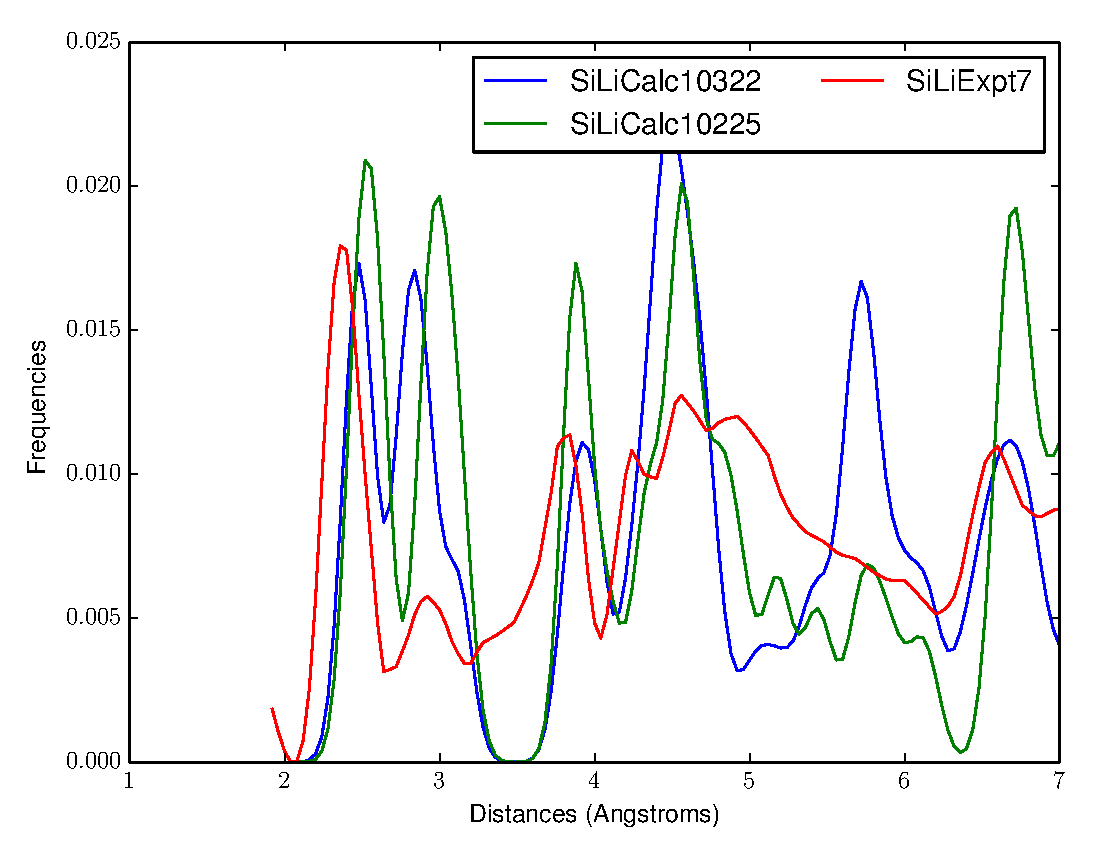
\includegraphics[scale=0.8]{figs/PC3MatchSiLiExpt7-SiLiCalc10225-SiLiCalc10322.eps}
    \caption{PCA Matches: SiLiExpt7, SiLiCalc10225, SiLiCalc10322}
  \end{center}
\end{figure}

\begin{figure}[ht]
  \begin{center}
    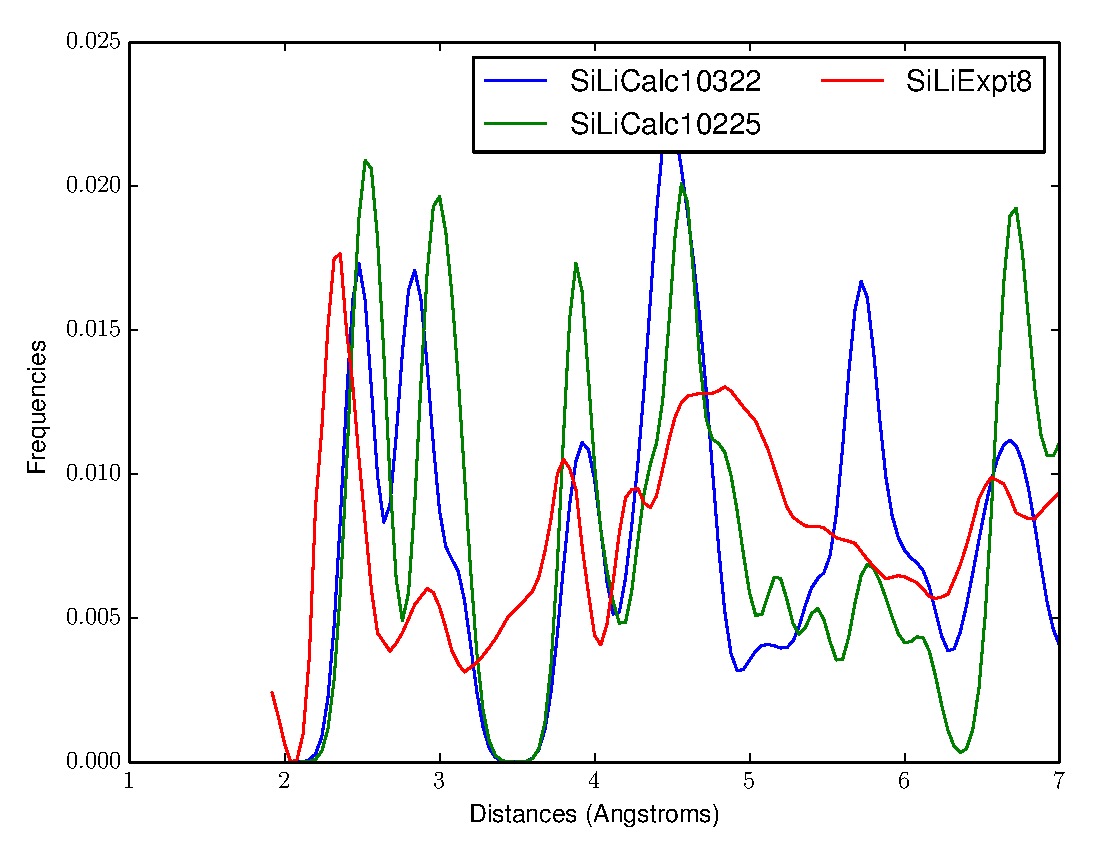
\includegraphics[scale=0.8]{figs/PC3MatchSiLiExpt8-SiLiCalc10225-SiLiCalc10322.eps}
    \caption{PCA Matches: SiLiExpt8, SiLiCalc10225, SiLiCalc10322}
  \end{center}
\end{figure}
\clearpage

\subsubsection{10 Principal Components}
\begin{table}[h]
\begin{center}
\begin{tabular}{|l|l|l|l|l|l|}
\hline
\textbf{Image}     & \textbf{Best Match} & \textbf{2}    & \textbf{3}             & \textbf{4}    & \textbf{5}    \\ \hline
\textbf{ExptGaAs}  & \textbf{CalcGaAs}   & SiLiCalc10329 & SiLiCalc11337          & SiLiCalc11436 & SiLiCalc10571 \\ \hline
\textbf{ExptInAs}  & SiLiCalc10646       & SiLiCalc10805 & SiLiCalc10792          & SiLiCalc10836 & SiLiCalc10767 \\ \hline
\textbf{SiLiExpt1} & SiLiCalc10213       & SiLiCalc10215 & \textbf{SiLiCalc10001} & SiLiCalc10003 & SiLiCalc10313 \\ \hline
\textbf{SiLiExpt2} & SiLiCalc10001       & SiLiCalc10003 & SiLiCalc10209          & SiLiCalc10317 & SiLiCalc10313 \\ \hline
\textbf{SiLiExpt3} & SiLiCalc10257       & SiLiCalc10317 & SiLiCalc10259          & SiLiCalc10258 & SiLiCalc10256 \\ \hline
\textbf{SiLiExpt4} & SiLiCalc10257       & SiLiCalc10258 & SiLiCalc10256          & SiLiCalc10229 & SiLiCalc10232 \\ \hline
\textbf{SiLiExpt5} & SiLiCalc10445       & SiLiCalc10616 & SiLiCalc11436          & SiLiCalc10329 & SiLiCalc11337 \\ \hline
\textbf{SiLiExpt6} & SiLiCalc10445       & SiLiCalc10616 & SiLiCalc11436          & SiLiCalc10693 & SiLiCalc11337 \\ \hline
\textbf{SiLiExpt7} & SiLiCalc10445       & SiLiCalc10693 & SiLiCalc11337          & SiLiCalc10616 & SiLiCalc10482 \\ \hline
\textbf{SiLiExpt8} & SiLiCalc10445       & SiLiCalc10693 & SiLiCalc10329          & SiLiCalc11337 & SiLiCalc10482 \\ \hline
\end{tabular}
  \caption{Recognition with 10 Principal Components}
  \end{center}
\end{table}

\begin{figure}[ht]
  \begin{center}
    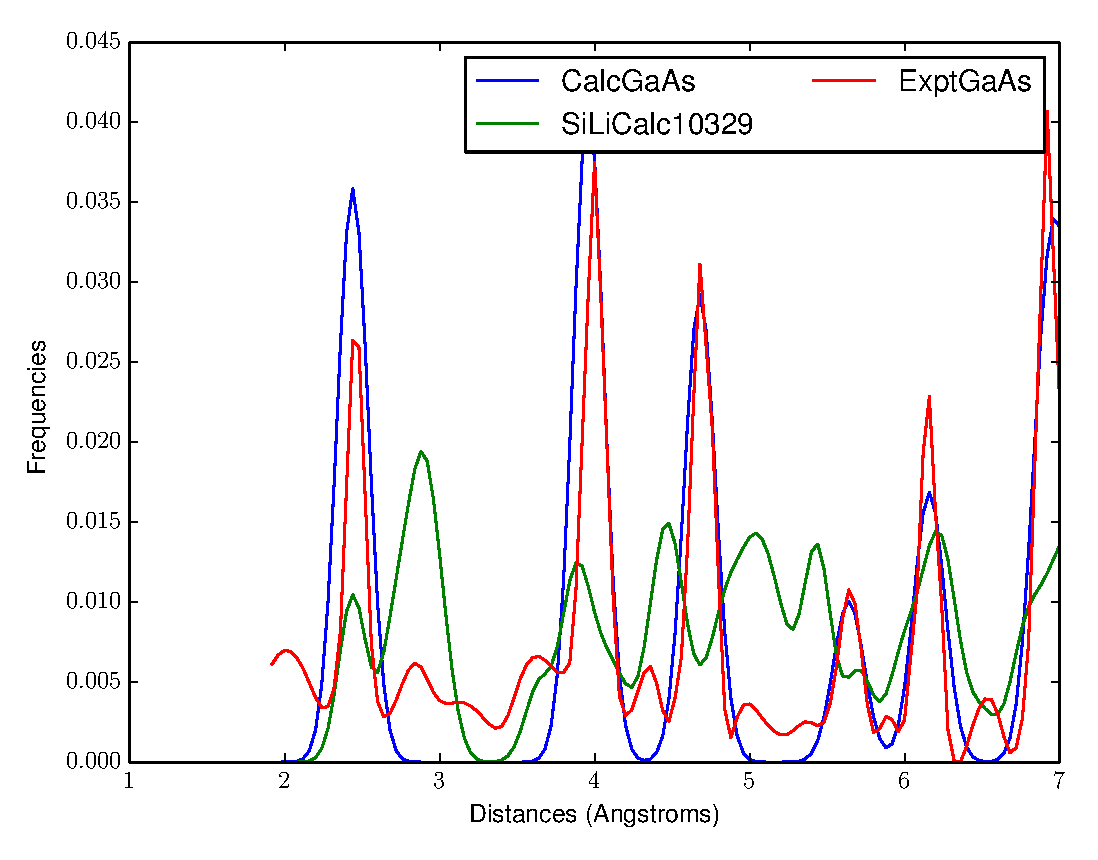
\includegraphics[scale=0.8]{figs/PC10MatchExptGaAs-CalcGaAs-SiLiCalc10329.eps}
    \caption{PCA Matches: ExptGaAs, CalcGaAs, SiLiCalc10329}
  \end{center}
\end{figure}

\begin{figure}[ht]
  \begin{center}
    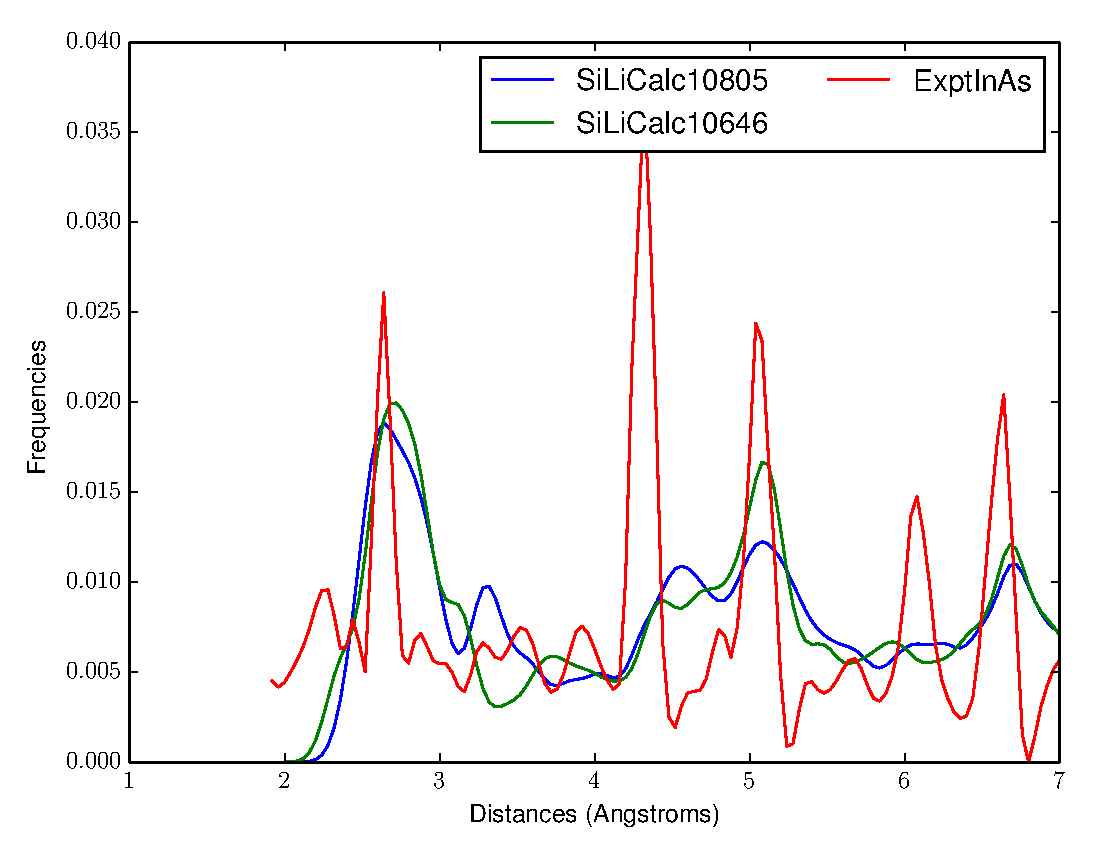
\includegraphics[scale=0.8]{figs/PC10MatchExptInAs-SiLiCalc10646-SiLiCalc10805.eps}
    \caption{PCA Matches: ExptInAs, SiLiCalc10646, SiLiCalc10805}
  \end{center}
\end{figure}

\begin{figure}[ht]
  \begin{center}
    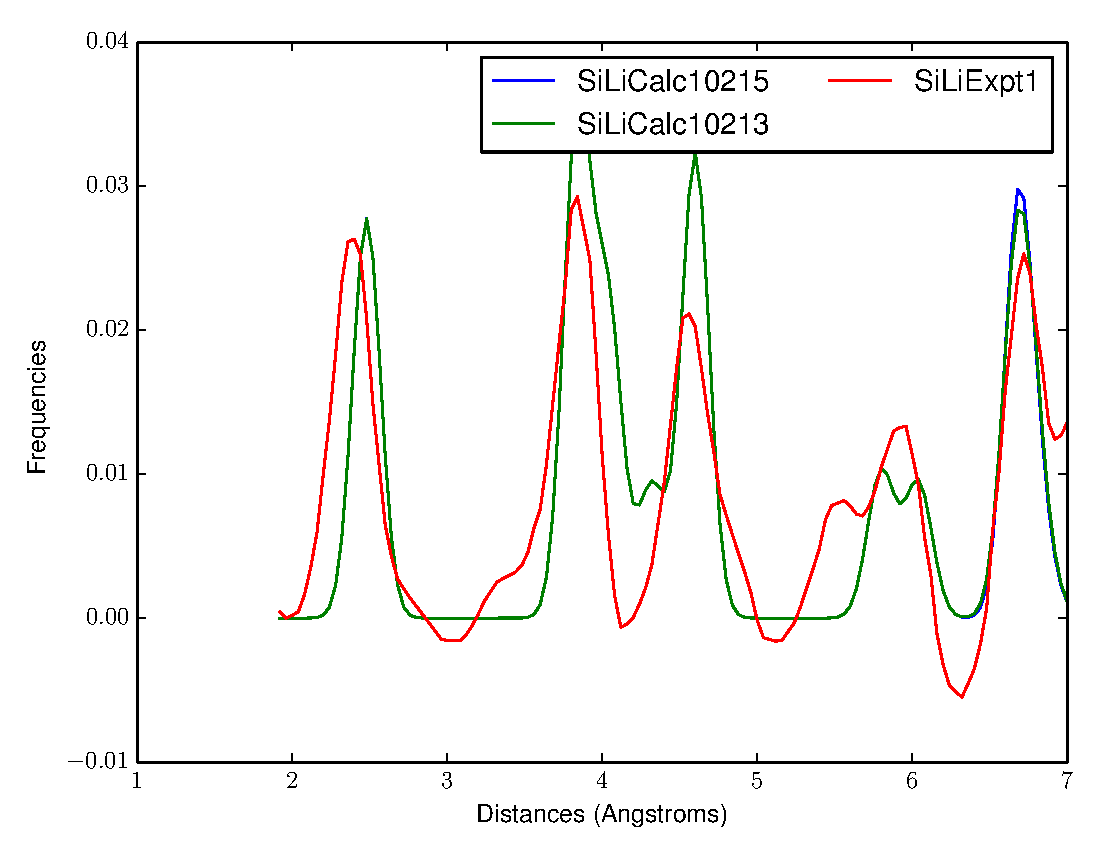
\includegraphics[scale=0.8]{figs/PC10MatchSiLiExpt1-SiLiCalc10213-SiLiCalc10215.eps}
    \caption{PCA Matches: SiLiExpt1, SiLiCalc10213, SiLiCalc10215}
  \end{center}
\end{figure}

\begin{figure}[ht]
  \begin{center}
    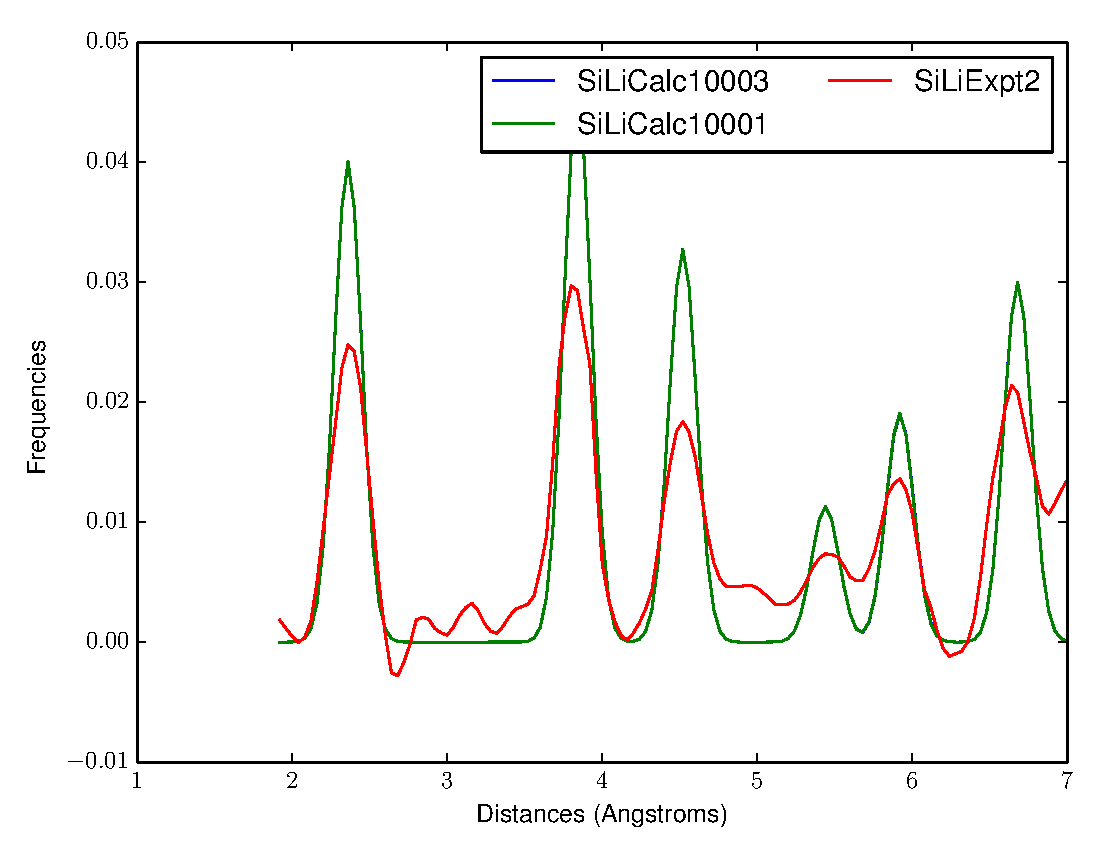
\includegraphics[scale=0.8]{figs/PC10MatchSiLiExpt2-SiLiCalc10001-SiLiCalc10003.eps}
    \caption{PCA Matches: SiLiExpt2, SiLiCalc10001, SiLiCalc10003}
  \end{center}
\end{figure}

\begin{figure}[ht]
  \begin{center}
    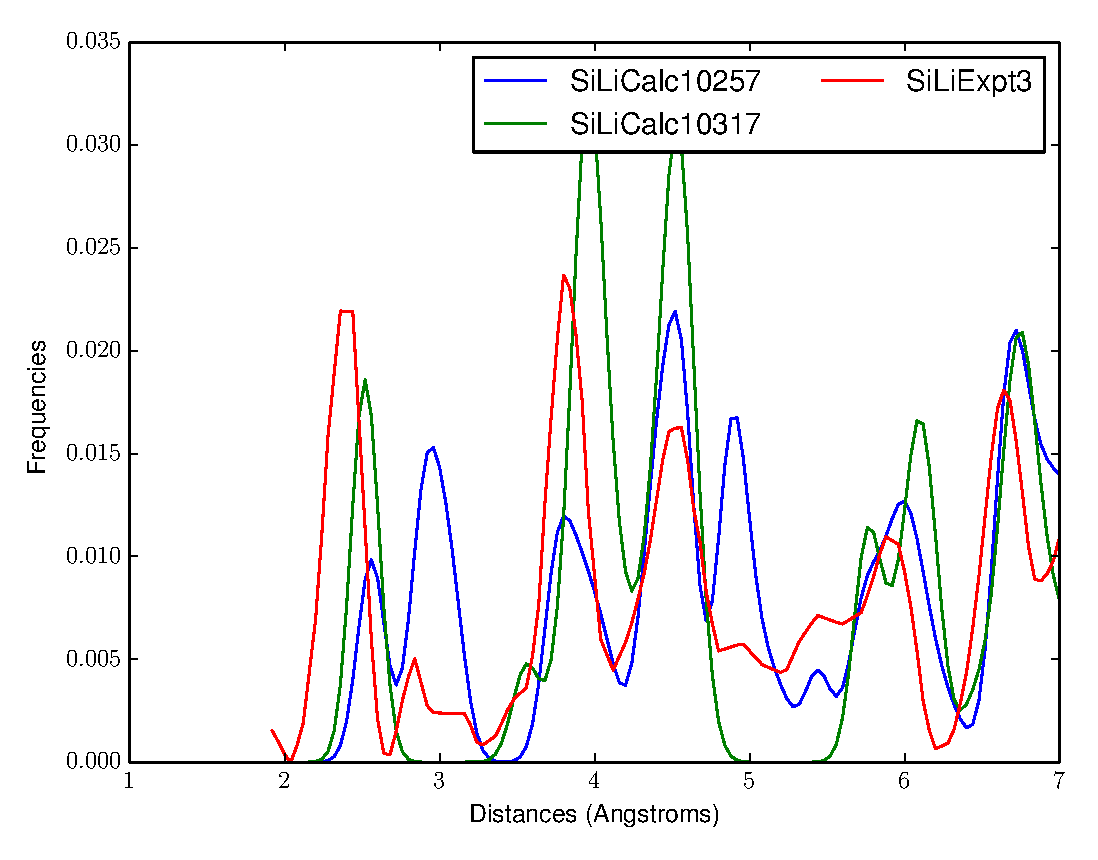
\includegraphics[scale=0.8]{figs/PC10MatchSiLiExpt3-SiLiCalc10257-SiLiCalc10317.eps}
    \caption{PCA Matches: SiLiExpt3, SiLiCalc10257, SiLiCalc10317}
  \end{center}
\end{figure}

\begin{figure}[ht]
  \begin{center}
    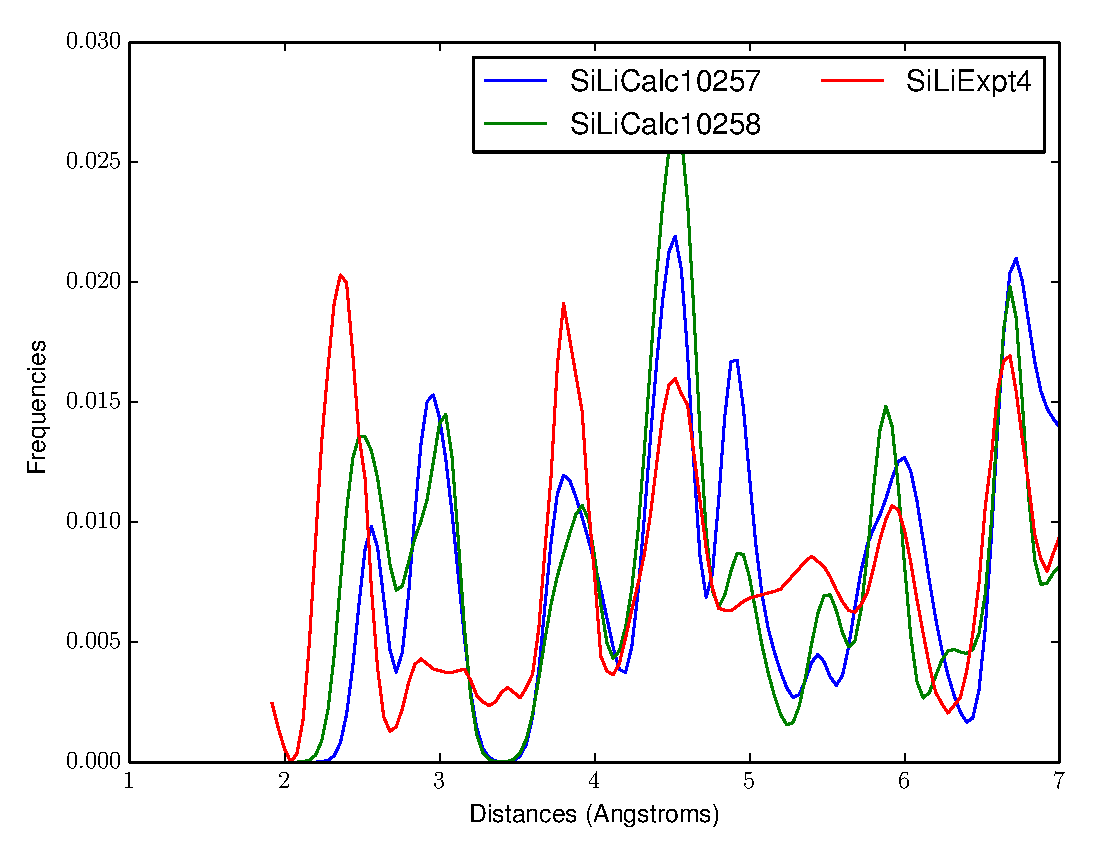
\includegraphics[scale=0.8]{figs/PC10MatchSiLiExpt4-SiLiCalc10257-SiLiCalc10258.eps}
    \caption{PCA Matches: SiLiExpt4, SiLiCalc10257, SiLiCalc10258}
  \end{center}
\end{figure}

\begin{figure}[ht]
  \begin{center}
    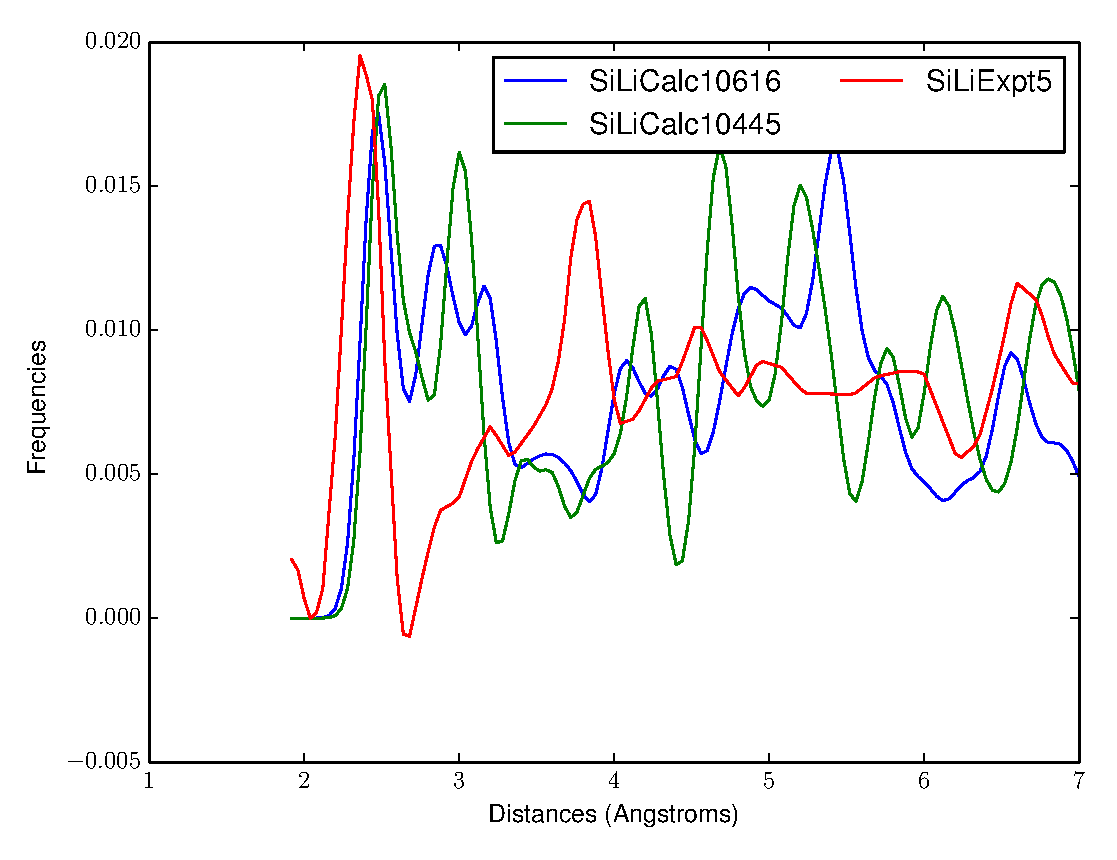
\includegraphics[scale=0.8]{figs/PC10MatchSiLiExpt5-SiLiCalc10445-SiLiCalc10616.eps}
    \caption{PCA Matches: SiLiExpt5, SiLiCalc10445, SiLiCalc10616}
  \end{center}
\end{figure}

\begin{figure}[ht]
  \begin{center}
    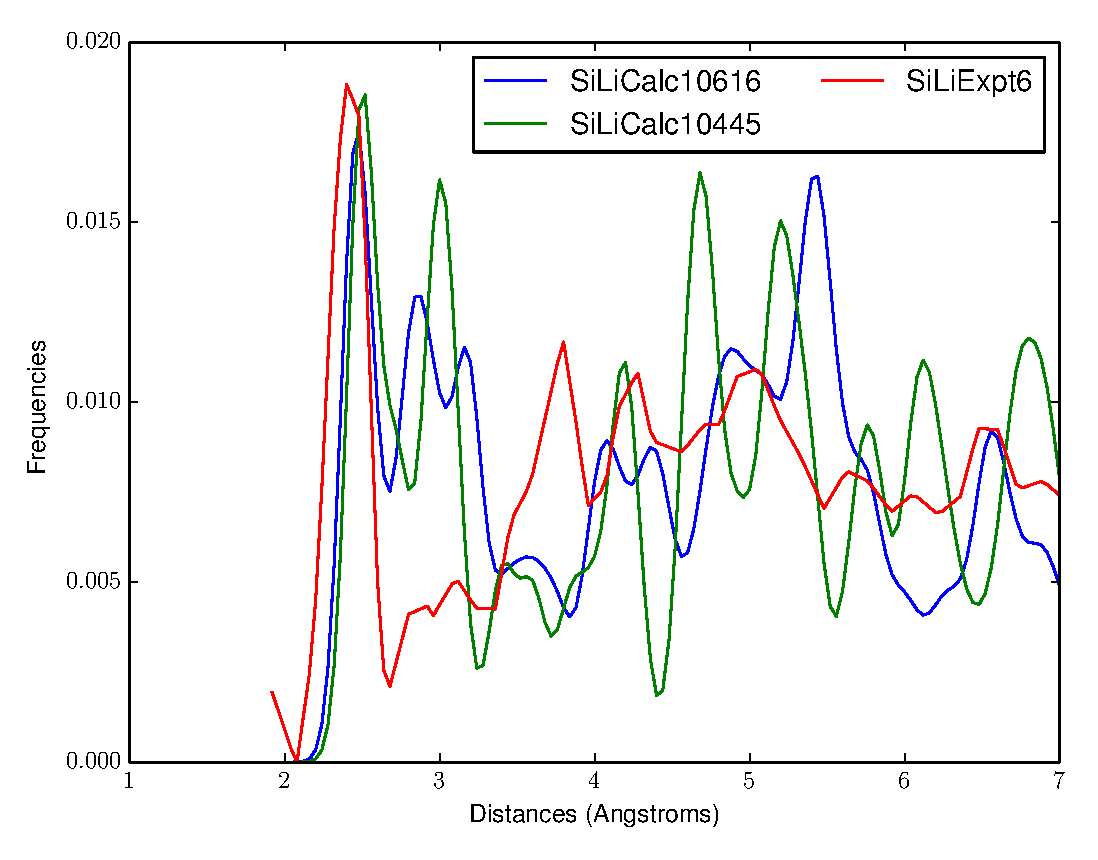
\includegraphics[scale=0.8]{figs/PC10MatchSiLiExpt6-SiLiCalc10445-SiLiCalc10616.eps}
    \caption{PCA Matches: SiLiExpt6, SiLiCalc10445, SiLiCalc10616}
  \end{center}
\end{figure}

\begin{figure}[ht]
  \begin{center}
    \includegraphics[scale=0.8]{figs/PC10MatchSiLiExpt7-SiLiCalc10445-SiLiCalc10693.eps}
    \caption{PCA Matches: SiLiExpt7, SiLiCalc10445, SiLiCalc10693}
  \end{center}
\end{figure}

\begin{figure}[ht]
  \begin{center}
    \includegraphics[scale=0.8]{figs/PC10MatchSiLiExpt8-SiLiCalc10445-SiLiCalc10693.eps}
    \caption{PCA Matches: SiLiExpt8, SiLiCalc10445, SiLiCalc10693}
  \end{center}
\end{figure}
\clearpage

\subsubsection{128 Principal Components}
\begin{table}[h]
\begin{tabular}{|l|l|l|l|l|l|}
\hline
\textbf{Image}     & \textbf{Best Match} & \textbf{2}             & \textbf{3}    & \textbf{4}    & \textbf{5}    \\ \hline
\textbf{ExptGaAs}  & \textbf{CalcGaAs}   & SiLiCalc10445          & SiLiCalc11436 & SiLiCalc10693 & SiLiCalc11337 \\ \hline
\textbf{ExptInAs}  & SiLiCalc10429       & SiLiCalc10602          & SiLiCalc10838 & SiLiCalc10901 & SiLiCalc10607 \\ \hline
\textbf{SiLiExpt1} & SiLiCalc10194       & \textbf{SiLiCalc10001} & SiLiCalc10003 & SiLiCalc10136 & SiLiCalc10147 \\ \hline
\textbf{SiLiExpt2} & SiLiCalc10001       & SiLiCalc10003          & SiLiCalc10194 & SiLiCalc10136 & SiLiCalc10147 \\ \hline
\textbf{SiLiExpt3} & SiLiCalc10258       & SiLiCalc10229          & SiLiCalc10245 & SiLiCalc11436 & SiLiCalc10259 \\ \hline
\textbf{SiLiExpt4} & SiLiCalc10258       & SiLiCalc11436          & SiLiCalc10229 & SiLiCalc11337 & SiLiCalc11634 \\ \hline
\textbf{SiLiExpt5} & SiLiCalc10616       & SiLiCalc11337          & SiLiCalc10693 & SiLiCalc11436 & SiLiCalc11336 \\ \hline
\textbf{SiLiExpt6} & SiLiCalc10616       & SiLiCalc10693          & SiLiCalc11337 & SiLiCalc11436 & SiLiCalc11336 \\ \hline
\textbf{SiLiExpt7} & SiLiCalc10693       & SiLiCalc11337          & SiLiCalc10482 & SiLiCalc10616 & SiLiCalc10651 \\ \hline
\textbf{SiLiExpt8} & SiLiCalc10693       & SiLiCalc10651          & SiLiCalc11337 & SiLiCalc10482 & SiLiCalc10616 \\ \hline
\end{tabular}
  \caption{Recognition with 128 Principal Components}
\end{table}

\begin{figure}[ht]
\begin{center}
\includegraphics[scale=0.8]{figs/PC128MatchExptGaAs-CalcGaAs-SiLiCalc10445.eps}
\caption{PCA Matches: ExptGaAs, CalcGaAs, SiLiCalc10445}
\end{center}
\end{figure}

\begin{figure}[ht]
\begin{center}
\includegraphics[scale=0.8]{figs/PC128MatchExptInAs-SiLiCalc10429-SiLiCalc10602.eps}
\caption{PCA Matches: ExptInAs, SiLiCalc10429, SiLiCalc10602}
\end{center}
\end{figure}

\begin{figure}[ht]
\begin{center}
\includegraphics[scale=0.8]{figs/PC128MatchSiLiExpt1-SiLiCalc10194-SiLiCalc10001.eps}
\caption{PCA Matches: SiLiExpt1, SiLiCalc10194, SiLiCalc10001}
\end{center}
\end{figure}

\begin{figure}[ht]
\begin{center}
\includegraphics[scale=0.8]{figs/PC128MatchSiLiExpt2-SiLiCalc10001-SiLiCalc10003.eps}
\caption{PCA Matches: SiLiExpt2, SiLiCalc10001, SiLiCalc10003}
\end{center}
\end{figure}

\begin{figure}[ht]
\begin{center}
\includegraphics[scale=0.8]{figs/PC128MatchSiLiExpt3-SiLiCalc10258-SiLiCalc10229.eps}
\caption{PCA Matches: SiLiExpt3, SiLiCalc10258, SiLiCalc10229}
\end{center}
\end{figure}

\begin{figure}[ht]
\begin{center}
\includegraphics[scale=0.8]{figs/PC128MatchSiLiExpt4-SiLiCalc10258-SiLiCalc11436.eps}
\caption{PCA Matches: SiLiExpt4, SiLiCalc10258, SiLiCalc11436}
\end{center}
\end{figure}

\begin{figure}[ht]
\begin{center}
\includegraphics[scale=0.8]{figs/PC128MatchSiLiExpt5-SiLiCalc10616-SiLiCalc11337.eps}
\caption{PCA Matches: SiLiExpt5, SiLiCalc10616, SiLiCalc11337}
\end{center}
\end{figure}

\begin{figure}[ht]
\begin{center}
\includegraphics[scale=0.8]{figs/PC128MatchSiLiExpt6-SiLiCalc10616-SiLiCalc10693.eps}
\caption{PCA Matches: SiLiExpt6, SiLiCalc10616, SiLiCalc10693}
\end{center}
\end{figure}

\begin{figure}[ht]
\begin{center}
\includegraphics[scale=0.8]{figs/PC128MatchSiLiExpt7-SiLiCalc10693-SiLiCalc11337.eps}
\caption{PCA Matches: SiLiExpt7, SiLiCalc10693, SiLiCalc11337}
\end{center}
\end{figure}

\begin{figure}[ht]
\begin{center}
\includegraphics[scale=0.8]{figs/PC128MatchSiLiExpt8-SiLiCalc10693-SiLiCalc10651.eps}
\caption{PCA Matches: SiLiExpt8, SiLiCalc10693, SiLiCalc10651}
\end{center}
\end{figure}

\clearpage

\subsection{Synthetic Experimental Image Recognition}
Here we run the alternative analysis approach outlined in section
\ref{s:algo_eval}. The exact method is described below.

\begin{verbatim}
For i = 1 to nSamples
  calculatedImage = randomlySelectFrom(calculatedImages)
  experimentalImage = addNoise(calculatedImage)
  bestMatchImage = findBestMatch(experimentalImage)

  If bestMatchImage == calculatedImage Then
    increment successCounter

Accuracy = successCounter / nSamples
\end{verbatim}

% TODO: how many principal components were used for this??
Below we consider findBestMatch functions that find the minimum L1 and L2 norm
in PCA space for ?all? principal components.

\begin{figure}[ht]
  \begin{center}
    \includegraphics[scale=0.8]{figs/accuracy_with_pca.png}
    \caption{Synthetic Experimental Images Accuracy}
  \end{center}
\end{figure}

Here we check how the accuracy varies as we increase the number of principal
components. We see that the accuracy does not change much after 15
principal components. This aligns with our conclusion from the cumulative
variance chart that 15 principal components are sufficient to describe much of
the variance in the data set.

\begin{figure}[ht]
  \begin{center}
    \includegraphics[scale=0.8]{figs/accuracy_by_num_pc.png}
    \caption{Accuracy vs Number of Principal Components}
  \end{center}
\end{figure}
\clearpage

\section{Recognition Using Sparse Representations}
Following the lead of Wright, et al. in "Robust Face Recognition via Sparse
Representation", we apply the method of recognition via sparse representation
to the xray images. The idea is that we try to express the experimental image as
a sparse linear combination of calculated images. If the solution is
sufficiently sparse, then the sparse solution can be found by minimizing the
$L_1$ norm of the coefficients.  The best match is then are the images that have
non-zero coefficients. One application of this that is outlined in Wright et
al's paper is to choose the best match as the image that produces the lowest
error after being multiplied by its coefficient.

\begin{align*}
\left(\begin{array}{ccccc}
c_{11} & c_{12} & c_{13} & \ldots & c_{1n} \\
\ldots & \ldots & \ldots & \ldots & \ldots \\
c_{m1} & c_{m2} & c_{m3} & \ldots & c_{mn} \\
\end{array}\right)
\left(\begin{array}{c}
y_1\\
y_2\\
y_3\\
\ldots\\
y_n\\
\end{array}
\right)
= \left(\begin{array}{c}
x_1\\
\ldots\\
x_m\\
\end{array}
\right)
+
\left(\begin{array}{c}
e_1\\
\ldots\\
e_m\\
\end{array}
\right)
\end{align*}

\begin{align*}
c_i&: i^{th} \mbox{ Calculated Image} \\
C &= [c_1 c_2 \cdots c_n] \\
x&: \mbox{Target Image}\\
\end{align*}

We wish to find the solution that is sparsest with bounded error. This can be
found via a second order cone programming problem.

\begin{align*}
\hat{y} = \underset{y}{\arg\min} \| y \|_1 \hspace{1em}|\hspace{1em} \|Cy - x\|_2 \leq \epsilon
\end{align*}

% TODO: rerun results with new smoothing coefficient
\subsection{Experimental Image Recognition}
!!! Need to rerun the results with the new smoothing coefficient. !!!
Here we show the best matches for the experimental images using the sparse
representation method. This method is able to recover the correct matches for
the known experimental and calculated pairs. The matches for most of the
experimental images seem reasonable as well. For SiLi experiments 6 through 8
though, the matches are quite bad.

\begin{table}[h]
  \begin{center}
  \begin{tabular}{|l|l|}
    \hline
    \textbf{Experiment} & \textbf{Match} \\ \hline
    ExptGaAs            & \textbf{CalcGaAs}       \\ \hline
    ExptInAs            & \textbf{CalcInAs}       \\ \hline
    SiLiExpt1           & \textbf{SiLiCalc10001}  \\ \hline
    SiLiExpt2           & SiLiCalc10001  \\ \hline
    SiLiExpt3           & SiLiCalc10001  \\ \hline
    SiLiExpt4           & SiLiCalc10003  \\ \hline
    SiLiExpt5           & SiLiCalc10003  \\ \hline
    SiLiExpt6           & SiLiCalc10616  \\ \hline
    SiLiExpt7           & SiLiCalc10382  \\ \hline
    SiLiExpt8           & SiLiCalc10382  \\ \hline
  \end{tabular}
  \caption{Experimental Image Recognition}
  \end{center}
\end{table}

\begin{figure}[ht]
  \begin{center}
    \includegraphics[scale=0.8]{figs/SparseRepExptGaAs-CalcGaAs.eps}
    \caption{ExptGaAs, CalcGaAs}
  \end{center}
\end{figure}

\begin{figure}[ht]
  \begin{center}
    \includegraphics[scale=0.8]{figs/SparseRepExptInAs-CalcInAs.eps}
    \caption{ExptInAs, CalcInAs}
  \end{center}
\end{figure}

\begin{figure}[ht]
  \begin{center}
    \includegraphics[scale=0.8]{figs/SparseRepSiLiExpt1-SiLiCalc10001.eps}
    \caption{SiLiExpt1, SiLiCalc10001}
  \end{center}
\end{figure}

\begin{figure}[ht]
  \begin{center}
    \includegraphics[scale=0.8]{figs/SparseRepSiLiExpt2-SiLiCalc10001.eps}
    \caption{SiLiExpt2, SiLiCalc10001}
  \end{center}
\end{figure}

\begin{figure}[ht]
  \begin{center}
    \includegraphics[scale=0.8]{figs/SparseRepSiLiExpt3-SiLiCalc10001.eps}
    \caption{SiLiExpt3, SiLiCalc10001}
  \end{center}
\end{figure}

\begin{figure}[ht]
  \begin{center}
    \includegraphics[scale=0.8]{figs/SparseRepSiLiExpt4-SiLiCalc10003.eps}
    \caption{SiLiExpt4, SiLiCalc10003}
  \end{center}
\end{figure}

\begin{figure}[ht]
  \begin{center}
    \includegraphics[scale=0.8]{figs/SparseRepSiLiExpt5-SiLiCalc10003.eps}
    \caption{SiLiExpt5, SiLiCalc10003}
  \end{center}
\end{figure}

\begin{figure}[ht]
  \begin{center}
    \includegraphics[scale=0.8]{figs/SparseRepSiLiExpt6-SiLiCalc10616.eps}
    \caption{SiLiExpt6, SiLiCalc10616}
  \end{center}
\end{figure}

\begin{figure}[ht]
  \begin{center}
    \includegraphics[scale=0.8]{figs/SparseRepSiLiExpt7-SiLiCalc10382.eps}
    \caption{SiLiExpt7, SiLiCalc10382}
  \end{center}
\end{figure}

\begin{figure}[ht]
  \begin{center}
    \includegraphics[scale=0.8]{figs/SparseRepSiLiExpt8-SiLiCalc10382.eps}
    \caption{SiLiExpt8, SiLiCalc10382}
  \end{center}
\end{figure}
\clearpage

\subsection{Synthetic Experimental Image Recognition}
Running the synthetic experimental image recognition analysis with the sparse
representation approach yields surprisingly bad results. Below the results are
plotted with different error bounds.
\begin{figure}[ht]
  \begin{center}
    \includegraphics[scale=0.8]{figs/SparseRepSynthExprAccuracy.png}
    \caption{Synthetic Experimental Image Recognition Accuracy}
  \end{center}
\end{figure}
\clearpage

\section{Code}
The code used to produce the results in this document as well as the document
itself can be found here: https://github.com/chadvoegele/xraysprectrapy

\section{Sources}
\begin{verbatim}
http://en.wikipedia.org/wiki/Atom_vibrations
http://en.wikipedia.org/wiki/Radial_distribution_function
http://en.wikipedia.org/wiki/Weierstrass_transform
http://matplotlib.org/api/mlab_api.html
http://en.wikipedia.org/wiki/Principal_components_analysis
First Principles Simulations of the Electrochemical Lithiation and Delithiation 
  of Faceted Crystalline Silicon
  Maria K. Y. Chan, C. Wolverton, and Jeffrey P. Greeley
  Journal of the American Chemical Society 2012 134 (35), 14362-14374
Pair Distribution Functions Analysis.
  Petkov, V. 2012. 
  Characterization of Materials. 1-14.
"Face recognition using eigenfaces,"
  Turk, M.A.; Pentland, A.P., 
  Computer Vision and Pattern Recognition, 1991. Proceedings CVPR '91., 
  IEEE Computer Society Conference on , vol., no., pp.586,591, 3-6 Jun 1991
"Robust Face Recognition via Sparse Representation," 
  Wright, J.; Yang, A.Y.; Ganesh, A.; Sastry, S.S.; Yi Ma, 
  Pattern Analysis and Machine Intelligence, IEEE Transactions on , 
  vol.31, no.2, pp.210,227, Feb. 2009
\end{verbatim}

\end{document}
